\chapter{Probability by Rosenthal}
In this chapter, I will include sporadic notes during my study of probability from the Rosenthal book. Also, I will try to compile a set of solutions for the problems in this book.



\section{Probability Triples}

\begin{definition}[Semialgebra]
	Let $ X $ be a set. A Semialgebra $ \mathcal{I} $ of the subsets of $ X $ is a collection of the subsets of such that 
	\begin{enumerate}[(a)]
		\item $ \emptyset, X \in \mathcal{I} $.
		\item $ \mathcal{I} $ is closed \emph{finite} \textbf{intersection}.
		\item For $ E \in \mathcal{I} $ it complement $ E^c $ can be written as a \emph{finite disjoint} \textbf{union} of sets in $ \mathcal{I} $.
	\end{enumerate}
\end{definition}
\begin{remark}
	One canonical example for a semialgebra is the set of all intervals in $ \R $, where the term interval contains all open, closed and half open intervals, as well as the empty set, singletons, and the whole space. 
\end{remark}

\begin{definition}[Algebra]
	Let $ \mathcal{M} $ be a collection of sets. Then $ \mathcal{M} $ is an algebra if 
	\begin{enumerate}[(a)]
		\item $ \Omega, \emptyset \in \mathcal{M} $
		\item $ \mathcal{M} $ is closed under complements.
		\item $ \mathcal{M} $ is closed under finite intersection.
		\item $ \mathcal{M} $ is closed under finite union.
	\end{enumerate}
\end{definition}

\begin{proposition}
	Let $ \mathcal{I} $ be a semialgebra, and $ \mathcal{F} = \sigma(\mathcal{I}) $. Let $ \mathbb{P},\mathbb{Q} $ be two probability measures defined on $ \mathcal{F} $. Then if $ \mathbb{P} $ agrees with $ \mathbb{Q} $ on $ \mathcal{I} $, then they agree on $ \mathcal{F} $.
\end{proposition}
\begin{remark}
	The condition that $ \mathcal{I} $ is a semialgebra is crucial. See \autoref{prob:BeingSemiAlgebraIsImportant} for an example.
\end{remark}


\newpage

\subsection{Solved Problems}
\begin{problem}
	Let $ \Omega = \set{1,.2,3,4} $. Determine whether or not each of the following is a $\sigma\text{-algebra}$.
	\begin{enumerate}[(a)]
		\item $ \mathcal{F}_1 = \set{\emptyset, \set{1,2},\set{3,4},\set{1,2,3,4}} $.
		\item $ \mathcal{F}_2 = \set{\emptyset,\set{3},\set{4},\set{1,2},\set{3,4},\set{1,2,3},\set{1,2,4},\set{1,2,3,4}} $.
		\item $ \mathcal{F}_3 = \set{\emptyset, \set{1,2},\set{1,3},\set{1,4},\set{2,3},\set{2,4},\set{3,4},\set{1,2,3,4}} $.
	\end{enumerate}
\end{problem}
\begin{solution}
	\begin{enumerate}[(a)]
		$ \, $
		\item $ \mathcal{F}_1  $ is a $\sigma\text{-algebra}$ and the set of its atoms are $ \set{\set{1,2},\set{3,4}} $. 
		\item $ \mathcal{F}_2 $ is a $\sigma\text{-algebra}$ and the set of its atoms are $ \set{\set{3},\set{4},\set{1,2}} $.
		\item $ \mathcal{F}_3 $ is \textbf{not} a $\sigma\text{-algebra}$ because $ \set{1,2},\set{2,3} \in \mathcal{F}_3 $ but $ \set{1,2}\cap\set{2,3} = \set{2} \notin \mathcal{F}_3 $.
 	\end{enumerate}
\end{solution}

\begin{problem}
	Let $ \Omega = \set{1,2,3,4} $, and let $ \mathcal{I} = \set{\set{1},\set{2}} $. Describe explicitly the $\sigma\text{-algebra}$ $ \sigma(\mathcal{I}) $ (i.e. the smallest $\sigma\text{-algebra}$ containing the collection $ \mathcal{I} $).
\end{problem}
\begin{solution}
	The smallest $\sigma\text{-algebra}$ containing the collection $ \mathcal{I} $ is
	\[ \sigma(\mathcal{I}) = \set{\set{1},\set{2},\set{3,4},\set{1,2},\set{2,3,4},\set{1,3,4},\set{1,2,3,4},\emptyset}. \]
	One way to check to see if this is really the smallest $\sigma\text{-algebra}$ is to first observe that the cardinality of $\sigma\text{-algebra}$ of a finite set should always be of the form $ 2^n $ for some $ n \in \N $, where $ n $ is the number of atoms (or the number of the non-empty sets the the $\sigma\text{-algebra}$ does not contain any of its subsets). Observe that $ \set{1} $ and $ \set{2} $ are already the atoms of the $\sigma\text{-algebra}$. Thus the size of $ \sigma(\mathcal{I}) $ must be at least four. However, we know that $ \sigma(\mathcal{I}) $ contains at least $ 5 $ elements (i.e. $ \set{1},\set{2},\set{1,2},\set{1,2,3,4},\emptyset $). This suggests that there should be at least one other atom in the set. Choosing that atom to be $ \set{3,4} $ will yield that $ \sigma(\mathcal{I}) $ that contains $ 8 $ elements. Since this already includes that collection $ \mathcal{I} $, and we can not have any smaller $\sigma\text{-algebra}$ then we are sure that this is the smallest $\sigma\text{-algebra}$.
\end{solution}


\begin{problem}
	Suppose $ \mathcal{F} $ is a collection of subsets of $ \Omega $, such that $ \Omega \in \mathcal{F} $.
	\begin{enumerate}[(a)]
		\item Suppose $ \mathcal{F} $ is an algebra. Prove that $ \mathcal{F} $ is a semialgebra.
		\item Suppose that whenever $ A,B \in \mathcal{F} $, then also $ A\backslash B \equiv A \cap B^c \in \mathcal{F} $. Prove that $ \mathcal{F} $ is an algebra. 
		\item Suppose that $ \mathcal{F} $ is closed under complement, and also closed under finite \emph{disjoint} unions. Give a counter example to show that $ \mathcal{F} $ might not be an algebra. 
	\end{enumerate}
\end{problem}

\begin{solution}
	\begin{enumerate}[(a)]
		\item Firstly, Since $ \mathcal{F} $ is an algebra, then it is closed under complement, hence $ \emptyset \in \mathcal{F} $. Secondly, Since it is closed under finite intersection, then it meets the closedness under finite intersection property of a semialgebra. Lastly, let $ E \in \mathcal{F} $. Since $ \mathcal{F} $ is an algebra then $ E^c \in \mathcal{F} $. So we can trivially write $ E^c = E^c $ as a finite disjoint union of sets in $ \mathcal{F} $. Thus $ \mathcal{F} $ is a semialgebra.
		\item Firstly, since $ \Omega \in \mathcal{F} $, then by hypothesis $ \Omega \backslash \Omega = \emptyset \in \mathcal{F} $. Secondly, let $ A \in \mathcal{F} $. Then by hypothesis $ \Omega \ A = A^c \in \mathcal{F} $, thus $ \mathcal{F} $ is closed under complement. Lastly, Let $ A,B \in \mathcal{F} $. By the reasoning above $ B^c \in \mathcal{F} $. And by hypothesis $ A\backslash B^c \in \mathcal{F} $. This implies that $ A \cap B \in \mathcal{F} $
		\item One simple counter example can be constructed when we let $ \Omega = \set{1,2,3,4} $ and then let 
		\[ \mathcal{F} = \set{\Omega,\emptyset, \set{1,2},\set{1,3},\set{1,4},\set{2,3},\set{2,4},\set{3,4}}. \]
		This collection is closed under finite disjoint union as well as complement. But it fails to be an algebra. For instance $ \set{1,2},\set{2,3} \in \mathcal{F} $, but their intersection is not in the collection.
	\end{enumerate}
\end{solution}

\begin{problem}
	Let $ \mathcal{F}_1,\mathcal{F}_2,\cdots $ be a sequence of collections of subsets of $ \Omega $, such that $ \mathcal{F}_n \subseteq \mathcal{F}_{n+1} $ for each $ n $. 
	\begin{enumerate}[(a)]
		\item Suppose that each $ \mathcal{F}_i $ is an algebra. Prove that $ \bigcup_{i=1}^\infty \mathcal{F}_i $ is also an algebra. 
		\item Suppose that each $ \mathcal{F}_i $ is a $\sigma\text{-algebra}$. Show (by counterexample) that $ \bigcup_{i=1}^\infty  \mathcal{F}_i$ need not be a $\sigma\text{-algebra}$.
	\end{enumerate}
\end{problem}
\begin{solution}
	\begin{enumerate}[(a)]
		\item Let $ \mathcal{G} = \bigcup_{i=1}^\infty \mathcal{F}_i $. First, observe that since $ \Omega, \emptyset \in \mathcal{F}_i $ for all $ i\in \N $ (since all of them are algebra), then it follows that $ \Omega, \emptyset \in \mathcal{G} $. Furthermore, let $ A \in \mathcal{G} $. Then $ A \in \mathcal{F}_i $ for some $ i\in\N $. Since $ \mathcal{F}_i $ is an algebra, then $ A^c \in \mathcal{F}_i $, hence $ A^c \in \mathcal{G} $. Lastly, let $ A,B \in \mathcal{G} $. Then $ A\in\mathcal{F}_i $ and $ B \in \mathcal{F}_j $ for some $ i,j \in \N $. WLOG we can assume $ i \leq j $. Then $ \mathcal{F}_i \subset \mathcal{F}_j $, hence $ A,B \in \mathcal{F}_j $. Since $ \mathcal{F}_j $ is an algebra, then $ A\cap B \in \mathcal{F}_j $. Thus $ A \cap B \in \mathcal{G} $. This proves that $ \mathcal{G} $ is an algebra. 
		\item Let $ \Omega = \N $. Let $ \mathcal{F}_n $ be the smallest $\sigma\text{-algebra}$ that contains the collection $ \set{\set{1},\cdots,\set{n}} $. On other way to think about $ \mathcal{F}_n $ is the $\sigma\text{-algebra}$ that contains the power set of $ \set{1,\cdots,n} $ as well as all of their complements (with respect to $ \Omega $). For instance, we have
		\[ \mathcal{F}_1 = \set{\emptyset,\set{1},\N, \set{1}^c}. \]
		Similarly
		\[ \mathcal{F}_2 = \set{\emptyset,\set{1},\set{2},\set{1,2},\N,\set{1}^c,\set{2}^c,\set{1,2}^c}, \]
		and etc. Let $ A_i = \set{2 i} $. Clearly $ A_i \in \bigcup_i \mathcal{F}_i $. However, $ \bigcup_i A_i \notin \bigcup_i \mathcal{F}_i$ as it does not belong to any $ \mathcal{F}_k $. Thus $ \bigcup_i\mathcal{F}_i $ is not a $\sigma\text{-algebra}$.
	\end{enumerate}
\end{solution}

\begin{problem}
	Suppose that $ \Omega = \N  $ is the set of positive integers, and $ \mathcal{F} $ is the set of all subsets $ A $ such that either $ A $ or $ A^c $ is finite, and $ \prob $ is defined by $ \prob(A) = 0 $ if $ A $ is finite, and $ \prob(A) = 1 $ if $ A^c $ is finite. 
	\begin{enumerate}[(a)]
		\item Is $ \mathcal{F} $ an algebra?
		\item Is $ \mathcal{F} $ a $\sigma\text{-algebra}$?
		\item Is $ \prob $ finitely additive?
		\item Is $ \prob $ countably additive on $ \mathcal{F} $, meaning that if $ A_1,A_2,\cdots \in \mathcal{F} $ are disjoint, and if it happens that $ \bigcup_n A_n \in \mathcal{F} $, then $ \prob(\bigcup_n A_n) = \sum_n \prob(A_n) $?
	\end{enumerate}
\end{problem}
\begin{solution}
	\begin{enumerate}[(a)]
		\item Yes. First, observe that $ \emptyset, \Omega \in \mathcal{F} $ as $ \emptyset $ is finite, and $ \Omega $ has a finite complement. Further, let $ A \in \mathcal{F} $. Then either it is finite or it has a finite complement, where for both cases we have $ A^c \in \mathcal{F} $. Let $ A_1,\cdots,A_n $ be a finite collection of sets in $ \mathcal{F} $. If all $ A_i $ for $ i=1,\cdots,n $ are finite, then since the finite intersection and complement of any finite collection of finite sets is finite, $ \bigcap_{i=1}^n A_i $ as well as $ \bigcup_{i=1}^n A_i$ are finite as well, thus belongs to $ \mathcal{F} $. If $ A_i $ are all infinite, then since they all belong to $ \mathcal{F} $ then they have finite complement, hence $ \bigcup_{i=1}^n A_i^c $ and $ \bigcap_{i=1}^n A_i^c $ are finite as well, thus belongs to $ \mathcal{F} $. If the collection is not in any of the case above, then there is $ 1\leq j \leq n $ such that $ A_j $ is finite. Thus $ \bigcup_i A_i $ is finite, thus belongs to $ \mathcal{F} $. Being closed under finite intersection and complements implies being closed under finite union.
		
		\item No. Let $ A_n = \set{2n} $. Then $ A_n \in \mathcal{F} $ for all $ n\in\N $. However, $ \bigcup_n A_n \notin \mathcal{F} $ as it is neither finite nor has a finite complement.
		
		\item Yes. First observe that if $ A,B $ are both infinite with $ A^c, B^c $ finite (this $ A,B \in \mathcal{F} $), then $ A\cap B \neq\emptyset $. Otherwise, $ A^c \cup B^c = \N $ which implies that either of them is infinite which is a contradiction. Thus given $ A,B $, if both are finite then $ \prob(A\cup B) = \prob(A) + \prob(B) = 0 $ as $ A\cup B $ is also finite. If both are infinite, then based on our argument above then they are not disjoint, so the argument of additivity does not apply to them. However if WLOG $ A $ is finite and $ B $ is infinite and $ A\cap B = 0 $, then $ A\cup B $ is also infinite thus $ 1 = \prob(A\cup B) = \prob(A) + \prob(B) = 0 + 1 $.
		
		\item No. Let $ A_n = \set{n} $. Then 
		\[ \prob(\bigcup_n A_n) = \prob(\N) = 1 \neq \sum_n \prob(A_n) = 0. \]
	\end{enumerate}
	
\end{solution}

\begin{proposition}
	Let $ \Omega = \N $ and let $ \mathcal{F} $ be the collection of all subsets of $ \Omega $ that is \emph{countable} or has countable \emph{complement}. Then $ \mathcal{F} = \sigma(\mathcal{A}) $ where $ \mathcal{A} = \set{\set{1},\set{2},\cdots} $, i.e. the set of all singletons.
\end{proposition}
\begin{proof}
	Let $ E \in \mathcal{F} $. First, note that the collection $ \mathcal{F} $ is a $\sigma\text{-algebra}$. Then, notice that $ \mathcal{F} $ contain $ \mathcal{A} $ as singletons are finite, hence countable. Since $ \sigma(\mathcal{A}) $ is the smallest $\sigma\text{-algebra}$ that contain $ \mathcal{A} $ then $ \sigma(\mathcal{A})\subset \mathcal{F} $. Let $ E \in \mathcal{F} $. Then $ E $ is either countable or has a countable complement. If $ E $ is countable then it can be written as a countable union of singletons in which each singleton contains one element of $ E $. Thus $ E \in \sigma(\mathcal{A}) $. If $ E^c $ is countable, then $ E^c $ can be written as a countable union of singleton of its element. By applying De Morgan's law $ E $ can be written as a countable union of the complements of singletons (which belong to $ \sigma(\mathcal{A}) $). Thus case also implies $ E \in \sigma(\mathcal{A}) $. Thus $ \mathcal{F} = \sigma(\mathcal{A}) $.
\end{proof}

\begin{problem}
	Suppose that $ \Omega = [0,1] $ is the unit interval, and $ \mathcal{F} $ is the set of all subsets $  A $ such that either $ A $ or $ A^c $ is finite, and $ \prob $ is defined by $ \prob(A) = 0 $ of $ A $ is finite and $ \prob(A) = 1 $ if $ A^c $ is finite. 
	\begin{enumerate}[(a)]
		\item Is $ \mathcal{F} $ an algebra?
		\item Is $ \mathcal{F} $ a $\sigma\text{-algebra}$?
		\item Is $ \prob $ finitely additive?
		\item Is $ \prob $ countably additive on $ \mathcal{F} $?
	\end{enumerate}
\end{problem}

\begin{solution}
	\begin{enumerate}[(a)]
		\item Yes. Being closed under complement is immediate from the definition. Thus $ \emptyset, \Omega \in \mathcal{F} $. Let $ A,B \in\mathcal{F} $. Then if $ A,B $ are both finite, then $ A\cap B $ is also finite thus $ A\cap B \in \mathcal{F} $. If $ A,B $ are both infinite, then $ A^c, B^c $ are both finite, so it is $ A^c \cup B^c $. Being closed under complement it implies that $ A\cup B  \in \mathcal{F}$. If one of $ A,B $ is infinite and the other one is finite, then $ A \cap B $ is finite, hence $ A\cap B \in \mathcal{F} $. Thus $ \mathcal{F} $ is a $\sigma\text{-algebra}$.
		\item No. Consider the collection $ \set{A_q}_{q \in \Q} $ where $ q \in A  $. Each of these sets are finite, hence $ A_q \in \mathcal{F} $ for all $ q \in \Q $. However $ \bigcup_q A_q $ is not finite and its complement is also not finite. Thus $ \mathcal{F} $ is not closed under countable union. 
		\item Yes. First observe that if $ A,B \in \mathcal{F} $ both infinite, then their intersection can not be empty, otherwise $ A^c \cup B^c = [0,1] $ which means that at least one of them is infinite which is a contradiction. With this in mind let $ A,B \in \mathcal{F} $. If $  A,B $ both finite with empty intersection then $ 0 = \prob(A\cup B) = \prob(A) + \prob(B) = 0 + 0 $ as $ A\cup B $ is also finite. If WLOG $ A $ is infinite and $ B $ is finite and $ A\cup B = \emptyset$, then $ A\cup B $ is also infinite and we have $ 1 = \prob(A\cup B) = \prob(A) + \prob(B) = 0 + 1 $. Thus $ \prob $ is finitely additive.
		\item Yes. First observe that we can not find any two $ A,B \in \mathcal{F} $ disjoint and infinite with empty intersection since then $ A^c\cup B^c = [0,1] $ that implies at least one of them is infinite. So let $ A_1,A_2,\cdots $ be a sequence of \emph{finite} sets in $ \mathcal{F} $. Then 
		\[ 0 = \prob(\bigcup_i A_i) = \sum_i \prob(A_i) = 0. \]
		In case if just one of $ A_i $ is infinite (no more than two can be infinite at the same time) then 
		$ \bigcup_i A_i  $ is infinite and 
		\[ 1 = \prob(\bigcup_i A_i) = \sum_i \prob(A_i) = 1.  \]
	\end{enumerate}
\end{solution}

\begin{problem}
	\label{prob:countableAdditivityOfProbabilityOnSigmaAlg}
	Suppose that $ \Omega =[0,1] $ is the unit interval, and $ \mathcal{F} $ is the set of all subsets $ A $ such that either $ A $ or $ A^c $ is countable (i.e. finite or countable), and $ \prob $ is defined by $ \prob(A) =0 $ if $ A $ is countable, and $ \prob(A) = 1 $ if $ A^c $ is countable.
	\begin{enumerate}[(a)]
		\item Is $ \mathcal{F} $ an algebra?
		\item Is $ \mathcal{F} $ a $\sigma\text{-algebra}$?
		\item Is $ \prob $ finitely additive?
		\item Is $ \prob $ countably additive?
	\end{enumerate}
\end{problem}
\begin{solution}
	\begin{enumerate}[(a)]
		\item Yes. Being closed under complement follows immediately from the definition. On the other hand, since $ \emptyset $ is finite, then $ \Omega $ (complement of the empty set) also belongs to $ \Omega $.  Let $ A,B \in \mathcal{F} $. If both are countable then $ A\cap B $ is also countable, thus $ A\cap B \in \mathcal{F} $. If for both their complement is countable, then $ A^c \cup B^c = (A\cap B)^c $ is countable. Thus $ A\cap B \in \mathcal{F} $. If one of them is countable, WLOG $ A $, then $ A\cap B $ is also countable, thus $ A\cap B \in \mathcal{F} $. Thus it is an algebra.  
		\item Yes. Being closed under complement follows from the definition and from this it follows that $ \Omega \in \mathcal{F} $. Let $ E_1,E_2,\cdots $ be a sequence of sets in $ \mathcal{F} $. If at least one of them is countable, then $ \bigcap_i E_i $ is also countable hence belonging to $ \mathcal{F} $. If all is uncountable, then $ \bigcup_i E^c_i $ is countable. We can write $ \bigcup_i E^c_i = (\bigcap_i E_i)^c $ that is finite. Thus $ \bigcap+i E_i \in \mathcal{F} $. This shows that $ \mathcal{F} $ is closed under countable union. Being closed under union follows from being closed under intersection and complement. Thus $ \mathcal{F} $ is a $\sigma\text{-algebra}$.
		\item Yes. We will show additivity for two sets and finite additivity will follow by induction. Let $ A,B \in \mathcal{F} $. If $ A,B $ both are disjoint countable then $ A\cup B $ is also countable. Thus $ 0= \prob(A\cup B) = \prob(A) + \prob(B) = 0+0 = 0 $. If $ A, B $ are both uncountable (i.e. $ A^c, B^c $ are countable) then $ A\cap B $ can not be non-empty, otherwise $ A^c\cup B^c = [0,1] $ which then implies that at least one of $ A^c $ or $ B^c $ be uncountable, which is a contradiction. When one of these sets is countable, WLOG $ A $, then $ A\cup B $ is also uncountable and we have $ 1 = \prob(A\cup B) = \prob(A) + \prob(B) = 1 + 0 $. Thus $ \prob $ is finitely countable.
		\item Yes. Let $ A_1,A_2,\cdots $ be a sequence of disjoint sets in $ \mathcal{F} $. Then at most one set can be uncountable, otherwise they will fail to be disjoint (see the reasoning in part (c)). If non of them are uncountable, then their union is also countable (countable union of countable sets is countable). Thus $ 0 = \prob(\bigcup_i A_i) = \sum_i \prob(A_i) = 0 $. If one of them is uncountable, then the union is also uncountable and we will have $ 1 = \prob(\bigcup_i A_i) = \sum_i \prob(A_i) = 0 +\cdots + 0 + 1 + 0 + \cdots = 1 $. Thus $ \prob $ is additive on $ \mathcal{F} $.
	\end{enumerate}
\end{solution}

\begin{problem}
	For the example of \autoref{prob:countableAdditivityOfProbabilityOnSigmaAlg}, is $ \prob $ uncountably additive?
\end{problem}
\begin{solution}
	No. Otherwise we can write $ \Omega = \bigcup_{x\in\Omega}\set{x} $. But we have
	\[ 1 = \prob(\Omega) = \sum_{x\in\Omega}\set{x} = 0. \]
\end{solution}

\begin{problem}
	Let $ \mathcal{F} $ be a $\sigma\text{-algebra}$, and write $ \abs{\mathcal{F}} $ for the total number of subsets in $ \mathcal{F} $. Prove that if $ \abs{\mathcal{F}}<\infty $, i.e. $ \mathcal{F} $  consists of just a finite number of subsets, then $ \abs{\mathcal{F}}=2^m $ for some $ m \in \N $. (\emph{Hint: Consider those non-empty subsets in $ \mathcal{F} $ which do not contain any other non-empty subset in $ \mathcal{F} $. How can all subsets in $ \mathcal{F} $ be build up from these particular subsets?}).
\end{problem}
\begin{solution}
	Let $ \mathcal{A} $ be the collection of all non-empty sets in $ \mathcal{F} $ whose non of its subsets do not belong to $ \mathcal{F} $. Then for any $ E \in \mathcal{F} $ can be build up from these ``atom'' by union. For each atom there are two possibilities to be present in the union or not. Thus there are in total $ 2^m $ elements in $ \mathcal{F} $.
\end{solution}


\begin{problem}
	\label{prob:BeingSemiAlgebraIsImportant}
	Let $ \Omega = \set{1,2,3,4} $, with $ \mathcal{F} $ the collection of all subsets of $ \Omega $. Let $ \mathbb{P} $ and $\mathbb{Q}$ be two probability measures on $ \mathcal{F} $ such that $ \mathbb{P}\set{1} = \mathbb{P}\set{2} = \mathbb{P}\set{3} = \mathbb{P}\set{4} = 1/4 $, and $ \mathbb{Q}\set{2} = \mathbb{Q}\set{4} = 1/2 $, extended to $ \mathcal{F} $ by linearity. Finally, let $ \mathcal{I}=\set{\emptyset,\Omega,\set{1,2},\set{2,3},\set{3,4},\set{1,4}} $.
	\begin{enumerate}[(a)]
		\item Prove that $ \mathbb{P}(A) = \mathbb{Q}(A) $ for all $ A \in \mathcal{I} $.
		\item Prove that there is $ A \in \sigma(\mathcal{I}) $ with $ \mathbb{P}(A) \neq \mathbb{Q}(A) $.
		\item Why does this not contradict Proposition 2.5.8 (in Rosenthal)?
	\end{enumerate}
\end{problem}
\begin{solution}
	\begin{enumerate}[(a)]
		\item By a simple calculation we can show the identity above. For instance
		\[ \mathbb{P}\set{1,2} = \mathbb{P}\set{1} + \mathbb{P}\set{2} = 1/4 + 1/4 = 1/2, \]
		where as
		\[ \mathbb{Q}\set{1,2} = \mathbb{Q}\set{1} + \mathbb{Q}\set{2} = 0 + 1/2 = 1/2. \]
		By a similar computation we can show
		\[ \mathbb{P}\set{2,3}=\mathbb{Q}\set{2,3}=1/2,\quad \mathbb{P}\set{3,4}=\mathbb{Q}\set{3,4}=1/2, \quad \mathbb{P}\set{1,4}=\mathbb{Q}\set{1,4}=1/2, \]
		and so on.
		
		\item First, observe that $ \set{1,2,3} \in \sigma(\mathcal{I}) $. That is because $ \set{3} = \set{2,3}\cap \set{3,4} \in \sigma(\mathcal{I}) $. Thus $ \set{1,2}\cup\set{3} = \set{1,2,3} \in \sigma(\mathcal{I}) $. But
		\[ \mathbb{P}\set{1,2,3} = 3/4, \qquad \mathbb{Q}\set{1,2,3} = 1/2. \]
		Thus if we let $ A = \set{1,2,3} \in \sigma(\mathcal{I}) $ then $ \mathbb{P}(A) \neq \mathbb{Q}(A) $.
		
		\item That is because the proposition 2.5.8 requires the collection $ \mathcal{I} $ be a semialgebra, which is not here. For instance $ \mathcal{I} $ is not closed under finite intersection as $ \set{1,2},\set{2,3} \in\mathcal{I} $ whereas their intersection is not in the collection.
	\end{enumerate}
\end{solution}

\begin{problem}
	Let $ (\Omega, \mathcal{M},\lambda) $ be Lebesgue measure on the interval $ [0,1] $. Let
	\[ \Omega' = \set{(x,y)\in \R^2: 0<x\leq 1, 0<y\leq 1}. \]
	Let $ \mathcal{F} $ be the collection of all subsets of $ \Omega' $ of the form
	\[ \set{(x,y)\in \R^2: x\in A, 0<y\leq 1} \]
	for some $ A \in \mathcal{M} $. Finally, defined a probability $ \mathbb{P} $ on $ \mathcal{F} $ by
	\[ \prob\set{(x,y)\in\R^2: x\in A, 0<y\leq 1} = \lambda(A). \]
	\begin{enumerate}[(a)]
		\item Prove that $ (\lambda', \mathcal{F},\prob) $ is probability space.
		\item Let $ \prob^* $ be the outer measure corresponding to $ \prob $ and $ \mathcal{F} $. Define the subset $ S \subseteq \Omega' $ by
		\[ S = \set{(x,y)\in \R^2: 0<x\leq 1, y = 1/2}. \]
		(Note that $ S \notin \mathcal{F} $.) Prove that $ \prob^*(S)=1 $ and $ \prob^*(S^c)=1 $.
	\end{enumerate}

\end{problem}
\begin{solution}
	\begin{enumerate}[(a)]
		\item $ \mathcal{F} $ being a $\sigma\text{-algebra}$ follows immediately from $ \mathcal{M} $ being a $\sigma\text{-algebra}$. To see this, for instance let $ H \in \mathcal{F} $. Then there exists some $ A \in \mathcal{M} $ such that $ H = A \times (0,1] $, where $ \times $ is the Cartesian product of two sets. Then $ H^c = \Omega'\backslash H $ will be given as $ H^c = A^c \times(0,1] $. Since $ A^c \in \mathcal{M} $ then it follows that $ H^c \in \mathcal{F} $. With a similar reasoning we can show that $ \mathcal{F} $ is a $\sigma\text{-algebra}$.
		
		\noindent Furthermore, $ \prob $ being a probability measure follows immediately from the fact that $ \lambda $ is a probability measure. For instance $ \prob(\Omega') = \lambda(\Omega) = 1 $, and $ \prob(B) \geq 0 $ for all $ B \in \mathcal{F} $ since we can write $ B = A \times(0,1] $ where $ A \in \mathcal{M} $ and by definition $ \prob(A) = \lambda(A) > 0 $. Countable additivity also follows from a similar line of reasoning.
		
		\item From the monotonicity of the outer measure and using the fact that $ S \subset \Omega' $ one gets that $ \prob^*(S) \leq \prob^*(\Omega') = \prob(\Omega') = 1 $. Furthermore, observe that we can write $ S = \Omega \times\set{1/2} $. Let $ \set{I_k \in \mathcal{F}} $ be any open cover for $ S $. Thus for each $ I_k $ there exists $ A_k \in\mathcal{M} $ such that $ I_k = A_k \times(0,1] $. Since $ S = \Omega\times\set{1/2} $ the  $ \set{B_k} $ will be an open cover for $ \Omega $. Using the fact that $ \prob(I_k) = \lambda(B_k) $
		\[ 1 = \lambda(\Omega)  \leq \sum_k \lambda(B_k) = \sum_k \prob(I_k)  \]
		Since the inequality above holds for any open cover $ \set{I_k} $ for $ S $ then we can conclude that $ 1 \leq \prob^*(S) $. So far
		\[ \prob^*(S) \geq 1, \qquad \prob^*(S)\leq 1. \]
		Then it follows that 
		\[ \prob^*(S) = 1. \]
	\end{enumerate}
\end{solution}

\begin{problem}
	\label{prob:ModifiedTHeorem}
	\begin{enumerate}[(a)]
		\item Where in the proof of Theorem 2.3.1 was assumption 2.3.3 used?
		\item How would the  of Theorem 2.3.1 be modified?
	\end{enumerate}
\end{problem}
\begin{solution}
	\begin{enumerate}[(a)]
		\item It is only used with proving the equality $ \prob(A) = \prob^*(A) $ for $ A \in \mathcal{I} $. I.e. to show that $ \prob^* $ is an extension of $ \prob $ to a larger domain $ \mathcal{M} $ which is a $\sigma\text{-algebra}$ that contain the collection $ \mathcal{I} $.
		\item Then the identity $ \prob^*(A) = \prob(A) $ for $ A \in \mathcal{I} $ should be replaced with $ \prob^*(A) \leq \prob(A) $.
 	\end{enumerate}
\end{solution}

\begin{problem}
	Let $ \Omega=\set{1,2} $, and let $ \mathcal{I} $ be the collection of all subsets of $ \Omega $, with $ \prob(\emptyset)=0, \prob(\Omega) = 1 $, and $ \prob\set{1}=\prob\set{2} = 1/3 $.
	\begin{enumerate}[(a)]
		\item Verify that all assumptions of theorem 2.3.1 other than 2.3.3 are satisfied.
		\item Verify that the assumption 2.3.3 is not satisfies.
		\item Describe precisely the $ \mathcal{M} $ and $ \prob^* $ that would result in this example from the modified version of Theorem 2.3.1 in \autoref{prob:ModifiedTHeorem}.
	\end{enumerate}
\end{problem}
\begin{solution}
	\begin{enumerate}[(a)]
		\item First, notice that the power set of $ \Omega $ finite, is always an algebra thus semialgebra. So $ \mathcal{I} $ is a semialgebra. On the other hand by the hypothesis we have $ \prob(\emptyset) = 0 $ and $ \prob(\Omega) = 1 $ which satisfies some of the conditions in Theorem 2.3.1. For the super-additivity, it holds because 
		\[ \prob(\set{1}\cup\set{2}) = 1 > \prob\set{1} + \prob\set{2} = 2/3. \]
		\item It is easy to check as $ \set{1,2},\set{1},\set{2} \in \mathcal{I} $ with $ \set{1,2} \subseteq \set{1}\cup \set{2} $ but
		\[ \prob\set{1,2} \not\leq \prob\set{1}+\prob\set{2}.\]
		\item {\color{red} \noindent TODO: TOBEADDED}
	\end{enumerate}
\end{solution}


\begin{problem}
	Let $ \Omega = [0,1] $. Let $ \mathcal{I}' $ be the set of all half-open intervals of the form $ (a,b], $ for $ 0\leq a < b \leq 1 $, togheter with the sets $ \emptyset, \Omega $, and $ \set{0} $.
	\begin{enumerate}[(a)]
		\item Prove that $ \mathcal{I}' $ is s semialgebra. 
		\item Prove that $ \sigma(\mathcal{I}') = \mathcal{B} $, i.e. that the $\sigma\text{-algebra}$ generated by this $ \mathcal{I}' $ is equal to the $\sigma\text{-algebra}$ generated by the $\sigma\text{-algebra}$ of (2.4.1) in Rosenthal.
		\item Let $ \mathcal{B}'_0 $ be the collection of all finite disjoint unions of elements of $ \mathcal{I}' $. Is $ \mathcal{B}'_0 $ the same as the algebra $ \mathcal{B}_0 $ defined in (2.2.4) Rosenthal?
	\end{enumerate}
\end{problem}
\begin{solution}
	\begin{enumerate}[(a)]
		\item By definition $ \mathcal{I}' $ contains $ \emptyset $ and $ \Omega $. To show being closed under intersection let $ A, B \in \mathcal{I}' $. If $ A,B $  are disjoint then $ A\cap B \in \mathcal{I'} $. However if $ A,B $ are not disjoint, then WLOG we can assume that $ A=(a_1,a_2], B = (b_1,b_2] $ where $ a_1 < b_1 < a_2 \leq b_2 $. Thus $ A\cap B = (b_1,a_2] $ which is also at $ \mathcal{I'} $. For the last property of a semialgebra, let $ A \in \mathcal{I'} $. We can assume $ A = (a,b] $ for $ 0\leq a<b \leq 1 $. Then $ A^c = [0,a] \cup (b,1] = \set{0}\cup (0,a] \cup (b,1] $ which is a finite disjoint union of elements of $ \mathcal{I'} $.
		\item By (2.4.1) Rosenthal, $ \mathcal{B} $ is the smallest $\sigma\text{-algebra}$ of all intervals in $ [0,1] $ where the term intervals include all open, closed, half-open, intervals as well as the empty set, singletons, and the whole set $ [0,1] $. First, notice that $ \sigma(\mathcal{I'}) $ contains all of the intervals in $ [0,1] $. That is because by using complements, countable unions, as well as countable intersections one can construct any kind of intervals using the intervals of the type $ (a,b] $. Since $ \mathcal{B} $ is the smallest $\sigma\text{-algebra}$ containing $ \mathcal{I} $ thus $ \sigma(\mathcal{I})\subseteq \sigma(\mathcal{I}') $. To show the equality,  observe that $ \mathcal{I'} \subset \mathcal{I} $ thus $ \sigma(\mathcal{I'}) \subseteq \sigma(\mathcal{I}) $. These two inequalities implies that $ \sigma(\mathcal{I'}) = \sigma(\mathcal{I}) = \mathcal{B}$. 
		\item No it is not. Since $ (1/3,1/2) \in \mathcal{B}_0 $ but not in $ \mathcal{B'}_0 $.
	\end{enumerate}
\end{solution}

\begin{problem}
	Let $ K $ be the Cantor set. Let $ D_n = K \oplus \frac{1}{n} $ be  a shifted Cantor set by $ 1/n $. Let $ B = \bigcup_n D_n $. 
	\begin{enumerate}[(a)]
		\item Draw a rough sketch of $ D_3 $.
		\item What is $ \lambda(D_3) $?
		\item Draw a rough image of $ B $.
		\item What is $ \lambda(B) $?
	\end{enumerate}
\end{problem}
\FloatBarrier
\begin{solution}
	\begin{enumerate}[(a)]
		\item See figure below.
		\item Since $ K \in \mathcal{B} $, then it is shift invariant, thus $ \lambda(K_3) = \lambda(K)  = 0 $.
		\item See the figure below.
		\item From the countable sub-additivity we have
		\[ \lambda(B) = \lambda(\bigcup_n K_n) \leq \sum_n \lambda(K_n) = 0. \]
	\end{enumerate}
	\begin{figure}[h!]
	
	
	\tikzset{every picture/.style={line width=0.75pt}} %set default line width to 0.75pt        
	
	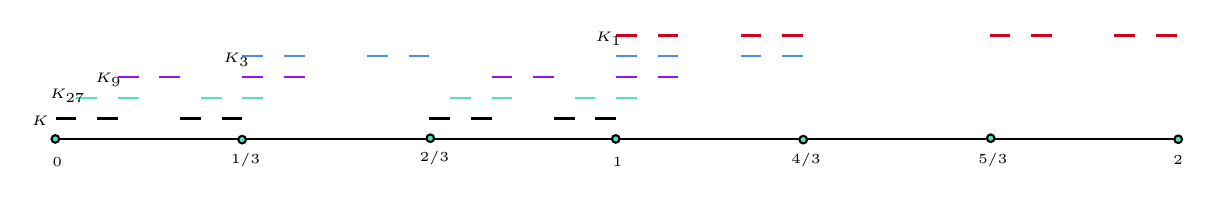
\begin{tikzpicture}[x=0.75pt,y=0.75pt,yscale=-1,xscale=1]
		%uncomment if require: \path (0,300); %set diagram left start at 0, and has height of 300
		
		%Straight Lines [id:da3663042093379123] 
		\draw    (70,160) -- (340,160) ;
		%Straight Lines [id:da30548704278309113] 
		\draw [color={rgb, 255:red, 144; green, 19; blue, 254 }  ,draw opacity=1 ][fill={rgb, 255:red, 144; green, 19; blue, 254 }  ,fill opacity=1 ]   (100,130) -- (110,130) ;
		%Straight Lines [id:da6192529867444463] 
		\draw [color={rgb, 255:red, 144; green, 19; blue, 254 }  ,draw opacity=1 ][fill={rgb, 255:red, 144; green, 19; blue, 254 }  ,fill opacity=1 ]   (120,130) -- (130,130) ;
		%Straight Lines [id:da9732533945560831] 
		\draw [color={rgb, 255:red, 144; green, 19; blue, 254 }  ,draw opacity=1 ][fill={rgb, 255:red, 144; green, 19; blue, 254 }  ,fill opacity=1 ]   (160,130) -- (170,130) ;
		%Straight Lines [id:da3271016125124977] 
		\draw [color={rgb, 255:red, 144; green, 19; blue, 254 }  ,draw opacity=1 ][fill={rgb, 255:red, 144; green, 19; blue, 254 }  ,fill opacity=1 ]   (180,130) -- (190,130) ;
		%Straight Lines [id:da21707011590164038] 
		\draw [color={rgb, 255:red, 144; green, 19; blue, 254 }  ,draw opacity=1 ][fill={rgb, 255:red, 144; green, 19; blue, 254 }  ,fill opacity=1 ]   (280,130) -- (290,130) ;
		%Straight Lines [id:da6944131266707991] 
		\draw [color={rgb, 255:red, 144; green, 19; blue, 254 }  ,draw opacity=1 ][fill={rgb, 255:red, 144; green, 19; blue, 254 }  ,fill opacity=1 ]   (300,130) -- (310,130) ;
		%Straight Lines [id:da4699188203805358] 
		\draw [color={rgb, 255:red, 144; green, 19; blue, 254 }  ,draw opacity=1 ][fill={rgb, 255:red, 144; green, 19; blue, 254 }  ,fill opacity=1 ]   (340,130) -- (350,130) ;
		%Straight Lines [id:da4206242986397042] 
		\draw [color={rgb, 255:red, 144; green, 19; blue, 254 }  ,draw opacity=1 ][fill={rgb, 255:red, 144; green, 19; blue, 254 }  ,fill opacity=1 ]   (360,130) -- (370,130) ;
		%Straight Lines [id:da18149657347980463] 
		\draw    (340,160) -- (610,160) ;
		%Shape: Circle [id:dp0666096192315917] 
		\draw  [fill={rgb, 255:red, 80; green, 227; blue, 194 }  ,fill opacity=1 ] (338,159.83) .. controls (338,158.82) and (338.82,158) .. (339.83,158) .. controls (340.85,158) and (341.67,158.82) .. (341.67,159.83) .. controls (341.67,160.85) and (340.85,161.67) .. (339.83,161.67) .. controls (338.82,161.67) and (338,160.85) .. (338,159.83) -- cycle ;
		%Shape: Circle [id:dp9884226065274095] 
		\draw  [fill={rgb, 255:red, 80; green, 227; blue, 194 }  ,fill opacity=1 ] (609,160) .. controls (609,158.99) and (609.82,158.17) .. (610.83,158.17) .. controls (611.85,158.17) and (612.67,158.99) .. (612.67,160) .. controls (612.67,161.01) and (611.85,161.83) .. (610.83,161.83) .. controls (609.82,161.83) and (609,161.01) .. (609,160) -- cycle ;
		%Shape: Circle [id:dp4266605000657435] 
		\draw  [fill={rgb, 255:red, 80; green, 227; blue, 194 }  ,fill opacity=1 ] (68,159.83) .. controls (68,158.82) and (68.82,158) .. (69.83,158) .. controls (70.85,158) and (71.67,158.82) .. (71.67,159.83) .. controls (71.67,160.85) and (70.85,161.67) .. (69.83,161.67) .. controls (68.82,161.67) and (68,160.85) .. (68,159.83) -- cycle ;
		%Straight Lines [id:da9770401267799609] 
		\draw    (70,150) -- (80,150) ;
		%Straight Lines [id:da04489044686774091] 
		\draw    (90,150) -- (100,150) ;
		%Straight Lines [id:da6941262785413165] 
		\draw    (130,150) -- (140,150) ;
		%Straight Lines [id:da5194844297129821] 
		\draw    (150,150) -- (160,150) ;
		%Straight Lines [id:da7760536614328373] 
		\draw    (250,150) -- (260,150) ;
		%Straight Lines [id:da3062585649045857] 
		\draw    (270,150) -- (280,150) ;
		%Straight Lines [id:da9561569076239738] 
		\draw    (310,150) -- (320,150) ;
		%Straight Lines [id:da058965052347594415] 
		\draw    (330,150) -- (340,150) ;
		%Straight Lines [id:da08135691890618824] 
		\draw [color={rgb, 255:red, 80; green, 227; blue, 194 }  ,draw opacity=1 ]   (80,140) -- (90,140) ;
		%Straight Lines [id:da9319257229221587] 
		\draw [color={rgb, 255:red, 80; green, 227; blue, 194 }  ,draw opacity=1 ]   (100,140) -- (110,140) ;
		%Straight Lines [id:da7931772700043691] 
		\draw [color={rgb, 255:red, 80; green, 227; blue, 194 }  ,draw opacity=1 ]   (140,140) -- (150,140) ;
		%Straight Lines [id:da9644967110186122] 
		\draw [color={rgb, 255:red, 80; green, 227; blue, 194 }  ,draw opacity=1 ]   (160,140) -- (170,140) ;
		%Straight Lines [id:da7254332920147846] 
		\draw [color={rgb, 255:red, 80; green, 227; blue, 194 }  ,draw opacity=1 ]   (260,140) -- (270,140) ;
		%Straight Lines [id:da9189177324927327] 
		\draw [color={rgb, 255:red, 80; green, 227; blue, 194 }  ,draw opacity=1 ]   (280,140) -- (290,140) ;
		%Straight Lines [id:da000462332081352157] 
		\draw [color={rgb, 255:red, 80; green, 227; blue, 194 }  ,draw opacity=1 ]   (320,140) -- (330,140) ;
		%Straight Lines [id:da36078056296552363] 
		\draw [color={rgb, 255:red, 80; green, 227; blue, 194 }  ,draw opacity=1 ]   (340,140) -- (350,140) ;
		%Straight Lines [id:da5133848731279023] 
		\draw [color={rgb, 255:red, 74; green, 144; blue, 226 }  ,draw opacity=1 ]   (160,120) -- (170,120) ;
		%Straight Lines [id:da4451939796286255] 
		\draw [color={rgb, 255:red, 74; green, 144; blue, 226 }  ,draw opacity=1 ]   (180,120) -- (190,120) ;
		%Straight Lines [id:da43204946632563] 
		\draw [color={rgb, 255:red, 74; green, 144; blue, 226 }  ,draw opacity=1 ]   (220,120) -- (230,120) ;
		%Straight Lines [id:da7906473674904837] 
		\draw [color={rgb, 255:red, 74; green, 144; blue, 226 }  ,draw opacity=1 ]   (240,120) -- (250,120) ;
		%Straight Lines [id:da04579659517201762] 
		\draw [color={rgb, 255:red, 74; green, 144; blue, 226 }  ,draw opacity=1 ]   (340,120) -- (350,120) ;
		%Straight Lines [id:da25232261478749574] 
		\draw [color={rgb, 255:red, 74; green, 144; blue, 226 }  ,draw opacity=1 ]   (360,120) -- (370,120) ;
		%Straight Lines [id:da034179599778776604] 
		\draw [color={rgb, 255:red, 74; green, 144; blue, 226 }  ,draw opacity=1 ]   (400,120) -- (410,120) ;
		%Straight Lines [id:da778496809035435] 
		\draw [color={rgb, 255:red, 74; green, 144; blue, 226 }  ,draw opacity=1 ]   (420,120) -- (430,120) ;
		%Straight Lines [id:da3950412348752457] 
		\draw [color={rgb, 255:red, 208; green, 2; blue, 27 }  ,draw opacity=1 ]   (340,110) -- (350,110) ;
		%Straight Lines [id:da9542539719446077] 
		\draw [color={rgb, 255:red, 208; green, 2; blue, 27 }  ,draw opacity=1 ]   (360,110) -- (370,110) ;
		%Straight Lines [id:da975939203402955] 
		\draw [color={rgb, 255:red, 208; green, 2; blue, 27 }  ,draw opacity=1 ]   (400,110) -- (410,110) ;
		%Straight Lines [id:da6837814611254798] 
		\draw [color={rgb, 255:red, 208; green, 2; blue, 27 }  ,draw opacity=1 ]   (420,110) -- (430,110) ;
		%Straight Lines [id:da1335307904306704] 
		\draw [color={rgb, 255:red, 208; green, 2; blue, 27 }  ,draw opacity=1 ]   (520,110) -- (530,110) ;
		%Straight Lines [id:da6855728787535145] 
		\draw [color={rgb, 255:red, 208; green, 2; blue, 27 }  ,draw opacity=1 ]   (540,110) -- (550,110) ;
		%Straight Lines [id:da26557145189620557] 
		\draw [color={rgb, 255:red, 208; green, 2; blue, 27 }  ,draw opacity=1 ]   (580,110) -- (590,110) ;
		%Straight Lines [id:da4074209351984093] 
		\draw [color={rgb, 255:red, 208; green, 2; blue, 27 }  ,draw opacity=1 ]   (600,110) -- (610,110) ;
		%Shape: Circle [id:dp983839454545631] 
		\draw  [fill={rgb, 255:red, 80; green, 227; blue, 194 }  ,fill opacity=1 ] (158,160.17) .. controls (158,159.15) and (158.82,158.33) .. (159.83,158.33) .. controls (160.85,158.33) and (161.67,159.15) .. (161.67,160.17) .. controls (161.67,161.18) and (160.85,162) .. (159.83,162) .. controls (158.82,162) and (158,161.18) .. (158,160.17) -- cycle ;
		%Shape: Circle [id:dp44575128451386936] 
		\draw  [fill={rgb, 255:red, 80; green, 227; blue, 194 }  ,fill opacity=1 ] (248.67,159.5) .. controls (248.67,158.49) and (249.49,157.67) .. (250.5,157.67) .. controls (251.51,157.67) and (252.33,158.49) .. (252.33,159.5) .. controls (252.33,160.51) and (251.51,161.33) .. (250.5,161.33) .. controls (249.49,161.33) and (248.67,160.51) .. (248.67,159.5) -- cycle ;
		%Shape: Circle [id:dp038392589885732686] 
		\draw  [fill={rgb, 255:red, 80; green, 227; blue, 194 }  ,fill opacity=1 ] (428.33,160.17) .. controls (428.33,159.15) and (429.15,158.33) .. (430.17,158.33) .. controls (431.18,158.33) and (432,159.15) .. (432,160.17) .. controls (432,161.18) and (431.18,162) .. (430.17,162) .. controls (429.15,162) and (428.33,161.18) .. (428.33,160.17) -- cycle ;
		%Shape: Circle [id:dp0834667196596044] 
		\draw  [fill={rgb, 255:red, 80; green, 227; blue, 194 }  ,fill opacity=1 ] (518.67,159.5) .. controls (518.67,158.49) and (519.49,157.67) .. (520.5,157.67) .. controls (521.51,157.67) and (522.33,158.49) .. (522.33,159.5) .. controls (522.33,160.51) and (521.51,161.33) .. (520.5,161.33) .. controls (519.49,161.33) and (518.67,160.51) .. (518.67,159.5) -- cycle ;
		
		% Text Node
		\draw (67,167.4) node [anchor=north west][inner sep=0.75pt]  [font=\tiny]  {$0$};
		% Text Node
		\draw (337,167.4) node [anchor=north west][inner sep=0.75pt]  [font=\tiny]  {$1$};
		% Text Node
		\draw (607,166.4) node [anchor=north west][inner sep=0.75pt]  [font=\tiny]  {$2$};
		% Text Node
		\draw (153,165.4) node [anchor=north west][inner sep=0.75pt]  [font=\tiny]  {$1/3$};
		% Text Node
		\draw (244,164.4) node [anchor=north west][inner sep=0.75pt]  [font=\tiny]  {$2/3$};
		% Text Node
		\draw (423,165.4) node [anchor=north west][inner sep=0.75pt]  [font=\tiny]  {$4/3$};
		% Text Node
		\draw (513,165.4) node [anchor=north west][inner sep=0.75pt]  [font=\tiny]  {$5/3$};
		% Text Node
		\draw (57,147.4) node [anchor=north west][inner sep=0.75pt]  [font=\tiny]  {$K$};
		% Text Node
		\draw (65.67,134.07) node [anchor=north west][inner sep=0.75pt]  [font=\tiny]  {$K_{27}$};
		% Text Node
		\draw (87.67,126.4) node [anchor=north west][inner sep=0.75pt]  [font=\tiny]  {$K_{9}$};
		% Text Node
		\draw (149.33,117.07) node [anchor=north west][inner sep=0.75pt]  [font=\tiny]  {$K_{3}$};
		% Text Node
		\draw (328.67,106.73) node [anchor=north west][inner sep=0.75pt]  [font=\tiny]  {$K_{1}$};
		
		
	\end{tikzpicture}
\end{figure}
	\FloatBarrier
\end{solution}
\begin{remark}
	Note that $ K \oplus K = \bigcup_{x\in K}( K \oplus x) = [0,2] $. I.e. the set of all numbers that can be created by adding two Cantor numbers is all the numbers in $ [0,2] $. Note that the Cantor set has Lebesgue measure zero, however $ [0,2] $ has measure 2. That is because $ \bigcup_{x\in K}) $ is in fact an uncountable union of sets (since a Cantor set is uncountable).
\end{remark}

\begin{problem}
	Let $ \Omega $ be a finite non-empty set, and let $ \mathcal{I} $ consist of all singletons in $ \Omega $, together with $ \emptyset $ and $ \Omega $. Let $ p: \Omega \to [0,1] $ with $ \sum_{\omega \in \Omega}p(\omega) = 1 $, and define $ \prob(\emptyset) = 0,\prob(\Omega) = 1 $, and $ \prob\set{\omega}=\prob(w) $ for all $ \omega \in \Omega $.
	\begin{enumerate}[(a)]
		\item Prove that $ \mathcal{I} $ is a semialgebra.
		\item Prove that (2.3.2) and $ (2.3.3) $ are satisfied. 
		\item Describe precisely the $ \mathcal{M} $ and $ \prob^* $ that result from applying Theorem 2.3.1 in Rosenthal.
		\item Are these $ \mathcal{M} $ and $ \prob^* $ the same as those described in Theorem 2.2.1 in Rosenthal?
 	\end{enumerate}
\end{problem}
\begin{solution}
	\begin{enumerate}[(a)]
		\item By definition $ \mathcal{I} $ contains $ \emptyset $ and well as $ \Omega $. $ \mathcal{I} $ is also closed under finite intersection as the intersection of two singletons is either a singleton or the empty set, and the intersection of $ \Omega $ with any singleton is a singleton. Furthermore, the intersection of any singleton with empty set is the empty set that is contained in $ \mathcal{I} $. Finally, let $ E \in \mathcal{I} $. If $ E $ is either $ \Omega $ or the empty set, then it complement can trivially be written as the disjoint union of $ \emptyset $ or $ \Omega $ respectively. If $ E $ is a singleton, then $ E^c $ can be written as the disjoint union of the singleton of its elements. Thus $ \mathcal{I} $ is a semialgebra.
		
		\item To check $ (2.3.2) $ let $ A_1,\cdots,A_k \in \mathcal{I} $ disjoint with $ \bigcup_i A_i \in \mathcal{I} $. Then $ \bigcup_i A_i = \Omega $ the collection $ A_i $'s are all of the singletons. Thus 
		\[ 1 = \prob(\bigcup_i A_i) = \prob(\Omega) = \sum_i \prob(A_i) = \sum_{\omega\in\Omega}\prob(\set{\omega}) = \sum_{\omega\in\Omega}p(\omega) = 1. \]
		Thus $ 2.3.2 $ holds with equality
		
		\noindent To verify $ (2.3.3) $ let $ A,A_1,A_2,\cdots,A_k \in \mathcal{I} $ with $ A \subset \bigcup_i A_i $. If $ A $ is empty set, then (2.3.3) holds as $ 0 \leq a $ for all $ a\in [0,1] $. If $ A $ is $ \Omega $, then the the sets $ A_i $ are the sets of all singletons. Thus 2.3.3 holds as $ 1\leq 1 $. Lastly, if $ A $ is a singleton, then at least one of $ A_i $'s should be the same as $ A $. Then $ \prob(A) \leq \prob(A_1) + \cdots + \prob(A_j) +  \cdots + \prob(A_k) $ for some $ 0\leq j \leq n $. Since $ \prob(A_j) = \prob(A) $ then 2.3.3 holds.
		
		\item The collection $ \mathcal{M} $ will be the same as the power set of $ \Omega $. And the probability measure $ \prob^* $ will be give as
		\[ \prob^*(A) = \sum_{\omega\in A} p(\omega). \]
		
		\item Although $ \mathcal{M} $ is the same as in theorem $ 2.3.1 $, but $ \prob^* $ is not the same. The probability measure defined in Theorem 2.3.1 is the uniform probability measure, where here it is not. The probability measure $ \prob^* $ is a more general one and will be the same as probability measure in Theorem 2.3.1 if we choose $ p(\omega) = 1/\abs{\Omega} $.
	\end{enumerate}
\end{solution}

\begin{problem}
	Let $ \prob $ and $ \mathbb{Q} $ be two probability measures defined on the same sample space $ \Omega $ and $\sigma\text{-algebra}$ $ \mathcal{F} $. 
	\begin{enumerate}[(a)]
		\item Suppose that $ \prob(A) = \mathbb{Q}(A) $ for all $ A \in \mathcal{F} $ with $ \prob(A) \leq 1/2 $. Prove that $ \prob = \mathbb{Q} $, i.e. that $ \prob(A) = \mathbb{Q}(A) $ for all $ A \in \mathcal{F} $.
		\item Give an example where $ \prob(A) = \qrob(A) $ for all $ A \in \mathcal{F} $ with $ \prob(A)<1/2 $, such that $ \prob \neq \qrob $, i.e. that $ \prob(A) \neq \qrob(A) $ for some $ A \in \mathcal{F} $.
	\end{enumerate}
\end{problem}
\begin{solution}
	\begin{enumerate}[(a)]
		\item Let $ A \in \mathcal{F} $ with $ \prob(A) > 1/2 $, hence $ \prob(A^c) \leq 1/2 $. Also, let $ E \in\mathcal{F} $ such that $ \prob(E)\leq 1/2 $. By definition (by using 2.3.7 or using the fact that $ \mathcal{F} $ is a $\sigma\text{-algebra}$ thus closed under intersection and complement) we can write
		\[ \prob(A) = \prob(A \cap E) + \prob(A\cap E^c). \]
		Observe that $ A\cap E \subseteq E $ thus by monotonicity $ \prob(A\cap E) \leq \prob(E) \leq 1/2 $. Further more, we can write $ \prob(A\cap E^c) = 1 - \prob(A^c \cup E) $. For the second term in the RHS we have
		\[ \prob(A^c \cup E) = \prob(A^c) + \prob(E) - \prob(A^c\cap E). \]
		Note that $ \prob(A^c)\leq 1/2 $ as well as since $ A^c\cap E \subset A^c $ thus by monotonicity $ \prob(A^c\cap E) \leq \prob(A^c) \leq 1/2 $. Thus
		\[ \prob(A) = \prob(A\cap E) + 1 - \prob(A^c) - \prob(E) + \prob(A^c\cap E). \]
		For all the terms in the RHS, since their measure with respect to $ \prob $ is less than oe equal to $ 1/2 $, thus $ \prob $ and $ \qrob $ agrees on them. Thus 
		\[ \prob(A) = \qrob(A\cap E) + 1 - \qrob(A^c) - \qrob(E) + \qrob(A^c\cap E) = \qrob(A). \]
		This completes the proof.
		
		\noindent \textbf{An easier solution}. Let $ A \in \mathcal{F} $ with $ \prob(A) > 1/2 $. Then $ \prob(A) = 1 - \prob(A^c) = 1 - \qrob(A^c) = \qrob(A) $, where we used the fact that $ \prob(A^c)\leq 1/2 $ thus $ \prob(A^c) = \qrob(A^c) $.
		
		\item Let $ \Omega =  \set{1,2} $ with $ \mathcal{F} $ being the power set of $ \Omega $. Then defined
		\[ \prob(\emptyset) = 0, \quad \prob(\set{1}) = \prob(\set{2}) = 1/2, \quad \prob(\set{1,2}) = 1. \]
		And
		\[ \qrob(\emptyset) = 0, \quad \qrob(\set{1}) = 1/10, \quad \qrob(\set{2})=9/10, \quad \qrob(\set{1,2}) = 1. \]
	\end{enumerate}
\end{solution}
\begin{remark}
	The hypothesis in part (a) in question above means that $ \prob $ and $ \qrob $ on all of the sets that has measure less than or equal to 1/2 w.r.t $ \prob $, must agree on all of the element of $ \mathcal{F} $.
\end{remark}

\begin{problem}
	Let $ (\Omega_1,\mathcal{F}_1,\prob_1) $ be Lebesgue measure on $ [0,1] $. Consider a second probability triple $ (\Omega_2, \mathcal{F}_2, \prob_2) $, defined as follows: $ \Omega_2 = \set{1,2} $, $ \mathcal{F}_2 $ consists of all subsets of $ \Omega_2 $, and $ \prob_2 $ is defined by $ \prob_2\set{1} = 1/3 $ and $ \prob_2\set{2} = 2/3 $, and additivity. Let $ (\Omega,\mathcal{F},\prob) $ be the product measure of $ (\Omega_1, \mathcal{F}_1, \prob_1) $ and $ (\Omega_2,\mathcal{F_2},\prob_2) $.
	\begin{enumerate}[(a)]
		\item Express each of $ \Omega, \mathcal{F} $ and $ \prob $ as explicitly as possible.
		\item Find a set $ A \in \mathcal{F} $ such that $ \prob(A) = 3/4 $.
	\end{enumerate}
\end{problem}
\begin{solution}
	\begin{enumerate}[(a)]
		\item The set $ \Omega $ is 
		\[ \Omega = \set{1,2}\times [0,1]. \]
		The collection $ \mathcal{F} $ is given by
		\[ \mathcal{F} = \set{\set{1}\times B: B \in\mathcal{B}}\quad \cup\quad \set{\set{2}\times B: B \in \mathcal{B}} \quad\cup\quad \set{\set{1,2}\times B: B \in \mathcal{B}}. \]
		And $ \prob $ is given by
		\[ \prob(\set{1}\times B) = \lambda(B)/3,\quad \prob(\set{2}\times B) = 2\lambda(B)/3,\quad \prob(\set{1,2}\times B) = \lambda(B). \]
		\item One easy choice for such a set would be $ A = \set{1,2}\times(0,3/4) $.
	\end{enumerate}
\end{solution}
\newpage


\section{Further Probabilistic Foundations}
\begin{definition}
	Let $ (\Omega,\mathcal{F},\prob) $ be a probability space and $ E_1,E_2 \in \mathcal{F} $ be two events. Then $ E_1 $ and $ E_2 $ are said to be independent events if and only if we have
	\[ \prob(E_1\cap E_2) = \prob(E_1)\prob(E_2). \]
	Another way to formulate this is to write
	\[ \prob(E_1 | E_2) = \prob(E_1). \]
\end{definition}
\begin{remark}
	The following diagram is very suggestive to make an intuition to see how does two independent events (i.e. sets) look like.
	\begin{figure}[h!]
	
	\centering
	% Pattern Info
	
	\tikzset{
		pattern size/.store in=\mcSize, 
		pattern size = 5pt,
		pattern thickness/.store in=\mcThickness, 
		pattern thickness = 0.3pt,
		pattern radius/.store in=\mcRadius, 
		pattern radius = 1pt}
	\makeatletter
	\pgfutil@ifundefined{pgf@pattern@name@_rptkzohuz}{
		\pgfdeclarepatternformonly[\mcThickness,\mcSize]{_rptkzohuz}
		{\pgfqpoint{0pt}{0pt}}
		{\pgfpoint{\mcSize+\mcThickness}{\mcSize+\mcThickness}}
		{\pgfpoint{\mcSize}{\mcSize}}
		{
			\pgfsetcolor{\tikz@pattern@color}
			\pgfsetlinewidth{\mcThickness}
			\pgfpathmoveto{\pgfqpoint{0pt}{0pt}}
			\pgfpathlineto{\pgfpoint{\mcSize+\mcThickness}{\mcSize+\mcThickness}}
			\pgfusepath{stroke}
	}}
	\makeatother
	
	% Pattern Info
	
	\tikzset{
		pattern size/.store in=\mcSize, 
		pattern size = 5pt,
		pattern thickness/.store in=\mcThickness, 
		pattern thickness = 0.3pt,
		pattern radius/.store in=\mcRadius, 
		pattern radius = 1pt}
	\makeatletter
	\pgfutil@ifundefined{pgf@pattern@name@_k41gami1g}{
		\pgfdeclarepatternformonly[\mcThickness,\mcSize]{_k41gami1g}
		{\pgfqpoint{0pt}{-\mcThickness}}
		{\pgfpoint{\mcSize}{\mcSize}}
		{\pgfpoint{\mcSize}{\mcSize}}
		{
			\pgfsetcolor{\tikz@pattern@color}
			\pgfsetlinewidth{\mcThickness}
			\pgfpathmoveto{\pgfqpoint{0pt}{\mcSize}}
			\pgfpathlineto{\pgfpoint{\mcSize+\mcThickness}{-\mcThickness}}
			\pgfusepath{stroke}
	}}
	\makeatother
	\tikzset{every picture/.style={line width=0.75pt}} %set default line width to 0.75pt        
	
	\begin{tikzpicture}[x=0.75pt,y=0.75pt,yscale=-1,xscale=1]
		%uncomment if require: \path (0,300); %set diagram left start at 0, and has height of 300
		
		%Shape: Rectangle [id:dp16467167448696318] 
		\draw   (110,80) -- (270,80) -- (270,200) -- (110,200) -- cycle ;
		%Shape: Circle [id:dp8792785092509503] 
		\draw  [pattern=_rptkzohuz,pattern size=6pt,pattern thickness=0.75pt,pattern radius=0pt, pattern color={rgb, 255:red, 80; green, 227; blue, 194}] (150,140) .. controls (150,117.91) and (167.91,100) .. (190,100) .. controls (212.09,100) and (230,117.91) .. (230,140) .. controls (230,162.09) and (212.09,180) .. (190,180) .. controls (167.91,180) and (150,162.09) .. (150,140) -- cycle ;
		%Shape: Rectangle [id:dp7768458786910091] 
		\draw  [pattern=_k41gami1g,pattern size=6pt,pattern thickness=0.75pt,pattern radius=0pt, pattern color={rgb, 255:red, 189; green, 16; blue, 224}] (190,80) -- (270,80) -- (270,200) -- (190,200) -- cycle ;
		
		% Text Node
		\draw (255.6,85.6) node [anchor=north west][inner sep=0.75pt]  [font=\footnotesize,color={rgb, 255:red, 0; green, 0; blue, 0 }  ,opacity=1 ]  {$A$};
		% Text Node
		\draw (157,132.4) node [anchor=north west][inner sep=0.75pt]  [font=\footnotesize,color={rgb, 255:red, 0; green, 0; blue, 0 }  ,opacity=1 ]  {$B$};
		% Text Node
		\draw (111,202.4) node [anchor=north west][inner sep=0.75pt]    {$\Omega $};
		
		
	\end{tikzpicture}
\end{figure}
	\FloatBarrier
	The intuition is that the proportion of $ A $ in the restricted world $ B $ (i.e. $ \prob(A|B) $) is the same as the proportion of $ A $ in the whole world. I.e.
	\[ \prob(A|B) = \frac{\prob(A\cap B)}{\prob(B)} = \frac{\prob(A)}{\prob(\Omega)} = \frac{\prob(A)}{1} = \prob(A). \]
\end{remark}

\begin{proposition}
	\label{prop:IndependentEvents}
	Let $ A,B $ be two independent events, i.e. $ \prob(A\cap B) = \prob(A) \prob(B) $. Then the pair of events, $ (A^c, B^c) $, $ (A^c,B) $, and $ (A,B^c) $ are also independent.
\end{proposition}
\begin{proof}
	We start by showing that $ A^c, B $ are independent events. Observe that
	\[ \prob(A^c\cap B) = 1 - \prob(A\cup B^c) = 1 - (\prob(B^c)+\prob(A\cap B)) = \prob(B) + \prob(A)\prob(B) = \prob(A^c) \prob(B). \]
	Thus $ A^c $ and $ B $ are independent events. Similarly we can prove that $ A,B^c $ are independent events. To show that the event $ A^c, B^c $ are independent we have
	\begin{align*}
		\prob(A^c\cap B^c) &= 1 - \prob(A\cup B) = 1 - \prob(A) - \prob(B) + \prob(A\cap B) = \prob(A^c) - \prob(B) + \prob(A)\prob(B) \\
		&= \prob(A^c)-\prob(B)(1-\prob(A)) = \prob(A^c)(1-\prob(B)) = \prob(A^c)\prob(B^c). 
	\end{align*}
	Thus $ A^c $ and $ B^c $ are independent.
\end{proof}

\begin{proposition}
	\label{prop:SeqIndependentEvents}
	Let $ A_1,A_2,\cdots $ be a sequence of independent events. Then the sequence of events $ B_1,B_2,\cdots $ are also independent where $ B_i $ is either equal to $ A_i $ or $ A_i^c $. In particular $ A_1^c, A_2^c,\cdots $ is a sequence of independent events.
\end{proposition}
\begin{proof}
 	Use the result of \autoref{prop:IndependentEvents} with Exercise 3.2.2 in Rosenthal.
\end{proof}
 
 
 \begin{observation}
 	Consider the following problem. Let $ A_1,A_2,\cdots, B_1,B_2,\cdots $ be events.
	\begin{enumerate}[(a)]
		\item Prove that 
		\[ (\limsup A_n) \cap (\limsup_n B_n) \supseteq \limsup_n (A_n\cap B_n). \]
		\item Give an example where the above inclusion is strict, and another example where it holds with equality.
	\end{enumerate}
 	Here, I will give a very intuitive explanation of the meaning of $ \limsup_n A_n $ as well as $ \limsup_n B_n $. Consider $ A_1,A_2,\cdots $ as sum lamps in a row that if $ w \in A_i $ then then $ i $th lamp turns on. Thus $ \limsup_n A_n $ are those elements in $ \Omega $ that if we evaluate its presence in the sequence of sets, a pattern will emerge where as you move further in the row of lamps you will still find a lamp that is on. Similarly for $ \limsup_n B_n $. However, the meaning of $ \omega \in (A_n\cap B_n) $ is that there is lamp position $ i $ such that this lamp is on for both $ A_n $ sequence and $ B_n $ sequence. Thus $ \limsup_n (A_n\cap B_n) $ is the set of all elements that if you evaluate its presence in the $ A_n $ sequence and $ B_n $ sequence, no matter how far you move in the sequence, you will still find spots where both lamps for $ A_i $ and $ B_i $ are on.
 \end{observation}
 
 \begin{proposition}[Borel-Cantelli Lemma]
 	Let $ A_1,A_2,\cdots \in \mathcal{F} $.
 	\begin{enumerate}[(a)]
 		\item If $ \sum_n \prob(A_n) < \infty $, then $ \prob(\limsup_n A_n) = 0 $.
 		\item If $ \sum_n \prob(A_n) = \infty $, and the events are \emph{independent}, then $ \prob(\limsup_n A_n) = 1 $.
 	\end{enumerate}
 \end{proposition}
 
\subsection{Solved Problems}
\[  \]
\begin{problem}
	Let $ X $ be a real-valued random variable defined on a probability triple $ (\Omega, \mathcal{F},\prob) $. Fill in the following blanks:
	\begin{enumerate}[(a)]
		\item $ \mathcal{F} $ is a collection of subsets of \blank.
		\item $ \prob(A) $ is a well-defined element of \blank provided that $ A $ is an element of \blank.
		\item $ \set{X\leq 5} $ is shorthand notation for the particular subset of \blank which is defined by \blank.
		\item If $ S $ is a subset of \blank, then $ \set{X\in S} $ is a subset of \blank.
		\item If $ S $ is a \blank subset of \blank, then $ \set{X \in S} $ must be a element of \blank.
	\end{enumerate}
\end{problem}
\begin{solution}
	$ \quad $
	\begin{enumerate}[noitemsep]
		\item $ \Omega $.
		\item $ \R $, $ \mathcal{F} $.
		\item $ \Omega $, $ \set{\omega\in \Omega: X(\omega)\leq 5} $.
		\item $ \mathcal{B} $, $ \mathcal{F} $.
		\item Borel, $ \R $, $\sigma\text{-algebra}$ $ \mathcal{F} $.
	\end{enumerate}
\end{solution}

\begin{problem}
	Let $ (\Omega, \mathcal{F},\prob) $ be Lebesgue measure on $ [0,1] $. Let $ A = (1/2,3/4) $ and $ B = (0,2/3) $. Are $ A $ and $ B $ independent events?
\end{problem}
\begin{solution}
	Yes. It is easy to check that  $ \prob(A \cap B) = \prob(A) \prob(B) $ holds for $ A,B $ as above.
\end{solution}


\begin{problem}
	Give an example of events $ A,B $, and $ C $, each of probability strictly between $ 0 $ and $ 1 $, such that 
	\begin{enumerate}[(a)]
		\item $ \prob(A\cap B) = \prob(A)\prob(B) $, $ \prob(A\cap C) = \prob(A)\prob(C) $, and $ \prob(B\cap C) = \prob(B)\prob(C)$; but it is not the case that $ \prob(A\cap B \cap C) = \prob(A)\prob(B)\prob(C) $.
		\item $ \prob(A\cap B) = \prob(A)\prob(B), \prob(A\cap C) = \prob(A)\prob(C) $, and $ \prob(A\cap B\cap C) = \prob(A)\prob(B)\prob(C) $; but it is not the case that $ \prob(B\cap C) = \prob(B)\prob(C) $.
	\end{enumerate}
\end{problem}
\begin{solution}
	\begin{enumerate}[(a)]
		\item Let $ \Omega = \set{a,b,c,d} $ and $ \prob $ a uniform discrete distribution on $ \Omega $. Let $ A = \set{a,b}, B = \set{a,c}, C = \set{a,d} $. Then we have 
		\[ \prob(A\cap B) = \prob(A\cap C) = \prob(B\cap C) = \prob(\set{a})=\frac{1}{4} = \prob(A)\prob(B) = \prob(A)\prob(C) = \prob(B)\prob(C). \]
		However, 
		\[ \prob(A\cap B\cap C) = \prob(\set{a}) \neq \prob(A)\prob(B)\prob(C) = \frac{1}{8}. \]
		\item Let $ \Omega = \set{1,2,3,4,5,6,7,8} $ and $ \prob $ a uniform discrete distribution on $ \Omega $. Define
		\[ A = \set{1,2,3,4}, \quad B = \set{3,4,5,6}, \quad C = \set{1,3,5,6}. \]
		Then we have $ \prob(A\cap B) = \prob(\set{3,4}) = \prob(A)\prob(B) = \frac{1}{4} $. Also $ \prob(A\cap C) = \prob(\set{1,3})=\prob(A)\prob(C) = \frac{1}{4} $. Furthermore $ \prob(A\cap B \cap C) = \prob(A)\prob(B)\prob(C) = \frac{1}{8} $. However $ \prob(B\cap C) = \prob(\set{3,5,6}) = \frac{3}{8} \neq \prob(B)\prob(C) = \frac{1}{4}$.
	\end{enumerate}
\end{solution}


\begin{problem}
	Suppose $ \set{A_n}\nearrow A $. Let $ f:\Omega\to \R $ be any function. Prove that $ \lim_{n\to\infty}\inf_{\omega\in A_n} f(\omega) = \inf_{\omega\in A}f(\omega) $.
\end{problem}
\begin{solution}
	Since $ \set{A_n}\nearrow A $ then $ A_1\subseteq A_2\subseteq \cdots $ with $ \bigcup_n A_n = A $. Let $ f(A_i) \subset \R $ denote the image of set $ A_i $ under the map $ f $. Then we have $ f(A_1)\subseteq f(A_2) \subseteq \cdots  $. Thus from properties of the infimum we have $ \inf f(A_1) \geq \inf f(A_2) \geq \cdots $. Observe that $ A_i \subset A $ for all $ i\in \N $, thus $ \inf(A_i)\geq \inf(A) $ for all $ i\in \N $. Thus the sequence of real numbers $ \set{\inf f(A_n)} $ is a decreasing sequence bounded from below. By monotone convergence theorem we conclude that $ \lim_{n\to\infty}f(A_n) $ exists. Then the next step is to show that this limit is the same as $ \inf f(A) $. Let $ \epsilon>0 $ given. Then there is $ \alpha\in f(A) $ such that $ \alpha < \inf f(A) + \epsilon $. Because $ f(A) = f(\bigcup_n A_n) = \bigcup_n f(A_n) $, then $ \exists m \in \N $ such that $ \alpha \in f(A_m) $. Then $ \inf f(A_m) \leq \alpha $. Thus $ \inf f(A_m) \leq \inf f(A) + \epsilon  $. Since we can find such $ A_m $ for every $ \epsilon>0 $, and since $ \inf f(A_n) $ is a decreasing sequence bounded below, then by the definition of limit we get
	\[ \lim_{n\to\infty} \inf_{A_n} f(A_n) = \inf_A f(A).  \]
\end{solution}

\begin{problem}
	Let $ (\Omega, \mathcal{F},\prob) $ be a probability triple such that $ \Omega $ is countable, and $ \mathcal{F} = 2^\Omega $. Prove that it is impossible for there to exist a sequence $ A_1,A_2,\cdots \in \mathcal{F} $ which is \emph{independent}, such that $ \prob(A_i)=\frac{1}{2} $ for each $ i $.
\end{problem}
\begin{solution}
	Let $ \omega \in \Omega $. Then define the sequence $ B_n $ as 
	\[ B_n = \begin{cases}
		A_n \qquad \omega \in A_n, \\
		A_n^c \qquad \omega \notin A_n.
	\end{cases} \]
	Then by \autoref{prop:SeqIndependentEvents} the sequence of events $ B_n $ are also independent. and we have $ \prob(B_n)=1/2 $ for all $ n $. By construction we have $ \omega \in \bigcap_n B_n $. Thus 
	\[ \prob(\set{\omega}) \leq \prob(\bigcap_n B_n) = \prod_n \prob(B_n) = \frac{1}{2^n} \]
	Since this is true for all $ n \in \N $ then $ \prob(\set{\omega}) = 0 $ for all $ \omega \in \Omega $. However, since $ \Omega $ is countable we have $ \Omega = \bigcup_{\omega \in \Omega}\set{\omega} $ which is a disjoint countable union. By countable additivity of the probability measure we have
	\[ 1 = \prob(\Omega) = \sum_{\omega\in\Omega}\prob(\omega) = 0,  \]
	which is a contradiction.
\end{solution}
\begin{solution}[A second solution!]
	Since $\mathbb{P}(A_i) = 1/2$ for all $i$, we have $\sum_i \mathbb{P}(A_i) = \infty$. Noting that $A_i$'s are independent then by Borel-Cantelli we have
	
	$$ \mathbb{P}(\{ A_n \ \text{i.o.} \}) = 1.$$
	
	Observe that $ \{ A_n \ \text{i.o.} \} \subseteq \Omega $, thus it is at most countable. So it can be written as a disjoint union of the singletons of its element. Applying the countable additivity of $\mathbb{P}$ will result in 1 = 0 which is a contradiction.
\end{solution}

\begin{problem}
	Let $ (\Omega,\mathcal{F},\prob) $ be the uniform distribution on $ \Omega = \set{1,2,3} $ as in Example 2.2.2. Give an example of a sequence $ A_1,A_2,\cdots\in\mathcal{F} $ such that 
	\[ \prob(\liminf_n A_n) < \liminf_n \prob(A_n) < \limsup_n \prob(A_n) < \prob(\limsup_n A_n). \]
\end{problem}
\begin{solution}
	An easy choice for such a sequence is 
	\[ \set{1},\set{1,2},\set{1,3},\set{2,3},\set{1},\set{1,2},\set{1,3},\set{2,3},\set{1},\cdots. \]
	It is easy to see that $ \liminf_n A_n = \emptyset, \limsup_n A_n = \set{1,2,3}, \liminf_n \prob(A_n) = 1/3$, and $ \limsup_n \prob(A_n) = 2/3 $. Thus we will get
	\[ \prob(\liminf_n A_n) < \liminf_n \prob(A_n) < \limsup_n \prob(A_n) < \prob(\limsup_n A_n). \]
\end{solution}

\begin{problem}
	Let $ \lambda $ be Lebesgue measure on $ [0,1] $, and let $ 0 \leq a \leq b \leq c\leq d \leq 1 $ be arbitrary real numbers. Give an example of a sequence $ A_1,A_2,\cdots $ of subsets of $ [0,1] $, such that $ \lambda(\liminf_f A_n) = a $, $ \liminf_f \lambda(A_n) = b $, $ \limsup_n \lambda(A_n) = c $, and $ \lambda(\limsup_n A_n) = d $. (\emph{Hint: Start with the case $ d = b + c - a $, which is easiest, and then carefully branch out from there.})
\end{problem}
\begin{solution}
	I am not sure how to use the hint, but one of the examples I could construct is considering the events
	\[ A_n = (\frac{1}{4}+\frac{1}{8}\sin(n), \frac{3}{4}-\frac{1}{8}\sin(n)). \]
	It is easy to see that
	\[ \limsup_n A_n = (\frac{1}{8},\frac{7}{8}),\quad  \liminf_n A_n = (\frac{3}{8},\frac{5}{8}). \]
	Thus we have
	\[ \lambda(\limsup_n A_n) = \frac{3}{4},\qquad \lambda(\liminf_n A_n) = \frac{1}{4}. \]
	Furthermore
	\[ \limsup_n\lambda(A_n) = \frac{3}{4},\quad \liminf_n\lambda(A_n) = \frac{1}{4}, \]
	Which satisfies the requirements.
\end{solution}

\begin{problem}
	Let $ A_1,A_2,\cdots, B_1,B_2,\cdots $ be events.
	\begin{enumerate}[(a)]
		\item Prove that 
		\[ (\limsup A_n) \cap (\limsup_n B_n) \supseteq \limsup_n (A_n\cap B_n). \]
		\item Give an example where the above inclusion is strict, and another example where it holds with equality.
	\end{enumerate}
\end{problem}
\begin{solution}
	\begin{enumerate}[(a)]
		\item Let $ \omega \in \limsup_n (A_n \cap B_n) $. Then $ \forall N > 0 $ there exists $ n > N $ such that $ \omega \in A_n\cap B_n $. By definition this implies that $ \omega \in (\limsup_n A_n \cap \limsup_n B_n) $, and this completes the proof.
		
		\item Fix $ \omega \in \Omega $. Let $ E $ be any set that contains $ \omega $. Let $ A_{2n} = E $ and $ A_{2n+1} = E^c $ for all $ n \in \N $. Furthermore let $ B_{2n} = E^c $ while $ B_{2n+1} = E $. By this construction we have
		\[ \set{\omega} \in \limsup_n A_n, \quad \set{\omega} \in \limsup_n B_n,\quad \text{thus}\quad \set{\omega} \in (\limsup_n A_n) \cap (\limsup_n B_n). \]
		However, since $ A_n \cap B_n = \emptyset $ for all $ n $ we have
		\[ \omega \notin \limsup_n (A_n \cap B_n), \]
		which shows the strict inequality of the inequality we proved in (a).
		
		To show an example which which the equality works, let $ E\subset\Omega $ by any subset. Define $ B_{bn} = A_{an} = E $ where $ (a,b)=1 $ (i.e. are relatively prime), and $ \emptyset $ otherwise. Then any $ \omega \in \limsup_n A_n $ will belong to one $ A_i $ every $ a $ sets, and by design will belong to $ B_i $ every $ b $ sets. Since $ (a,b)=1 $, then these sets will be the same infinitely often, hence $ \omega \in \limsup(A_n\cap B_n) $ as well.
	\end{enumerate}
\end{solution}

\begin{problem}
	Let $ A_1,A_2,\cdots $ be a sequence of events, and let $ N \in \N $. Suppose there are events $ B,C $ such that $ B\subseteq A_n \subseteq C $ for all $ n\geq N $, and such that $ \prob(B) = \prob(C) $. Prove that $ \prob(\liminf_n A_n) = \prob(\limsup_n A_n) = \prob(B) = \prob(C) $.
\end{problem}
\begin{solution}
	We claim 
	\[ B \subseteq \limsup_n A_n \subseteq C, \qquad B \subseteq \liminf_n A_n \subseteq C. \]
	To show the first statement, let $ \omega \in B $. Then since for all $ n $ large enough we have $ B \subseteq A_n \subseteq C $, we have $ B \in A_n $, thus $ B \subseteq \limsup_n A_n $. Furthermore, let $ \omega \in \limsup_n A_n $. Then for all $ N $ we can find $ n>N $ such that $ \omega\in A_n $. By hypothesis $ \omega\in C $. Thus $ \limsup_n A_n \subseteq C $.
	
	\noindent To show the second statement, let $ \omega \in C $. Then since for all $ n $ large enough $ B \subseteq A_n \subseteq C $ we see that $ B\subseteq \liminf_n A_n \subseteq C $. By the monotonicity of the probability we have
	\[ \prob(B) \leq \prob(\limsup_n A_n) \leq \prob(C) ,\qquad \prob(B)\leq \prob(\liminf_n A_n)\leq \prob(C).\]
	Since $ \prob(B) = \prob(C) $ then we conclude that 
	\[ \prob(\limsup_n A_n) = \prob(\liminf_n A_n) = \prob(B) = \prob(C). \]
\end{solution}


\begin{problem}
	Let $ \set{X_n} $ be independent random variables, with $ \prob(X_n = i) = 1/n $ for $ i=1,2,3,\cdots, n $. Compute $ \prob(X_n = 5\ i.o.) $, the probability that an infinite number of the $ X_n $ are equal to $ 5 $.
\end{problem}
\begin{solution}
	Let $ A_n = \set{X_n = 5} $. Then by hypothesis $ \prob(A_n) = 0 $ for $ n < 5 $ and $ \prob(A_n) = 1/n $ for $ n \geq 5 $. Thus $ \sum_n \prob(A_n) = \infty $. As the random variables $ X_n $ are all independent, so is the events $ A_n $. Thus using the Borel-Cantelli Lemma we conclude that $ \prob(A_n\ i.o.) = 1 $.
\end{solution}


\begin{problem}
	Let $ X $ be a random variable with $ \prob(X>0)>0 $. Prove that there exists $ \delta>0 $ such that $ \prob(X \geq \delta) > 0 $. (\emph{Hint: Use the continuity of the probability function})
\end{problem}
\begin{solution}
	Let $ A = \set{X>0} $, and consider the events $ A_n = \set{X > 1/n} $. Observe that $ \set{A_n}\nearrow A $. The sequence of real numbers $ \set{\prob(A_n)} $ is an increasing sequence (by the monotonicity) and is converging to $ \prob(A) $ (by the continuity). Let $ \epsilon = \prob(A)/2 $. Then by the definition of the convergence of real numbers for all $ N>0 $ we have $ \epsilon < \prob(A_n) $ for all $ n>N $. Let $ \delta = 1/N $. This completes the proof.
\end{solution}


\begin{problem}
	Let $ X_1,X_2,\cdots $ be defined jointly on some probability space $ (\Omega,\mathcal{F},\mathcal{P}) $, with $ \sum_{i=1}^{\infty}i^2\prob(i \leq X_n < i+1) \leq C <\infty $ for all $ n $. Prove that $ \prob(X_n \geq n\ i.o.) = 0 $.
\end{problem}
\begin{solution}
	Observe that
	\begin{align*}
		C &\geq \sum_{i=1}^{\infty}i^2\prob(i\leq X_n < i+1) \\
		&\geq \sum_{i=n}^{\infty}i^2\prob(i\leq X_n < i+1) \\
		&\geq n^2 \sum_{i=n}^{\infty}\prob(i\leq X_n<i+1) \\
		&= n^2 \prob(X_n \geq n).
	\end{align*}
	Thus we have $ \prob(X_n\geq n) \leq C/n^2 $. Since $ C/n^2 $ is summable, and the probability function is positive, then $ \prob(X_n \geq n) $ is also summable. I.e.
	\[ \sum_n \prob(X_n \geq n) < \infty. \]
	Using Borel-Cantelli lemma we then have
	\[ \prob(X_n \geq n\ i.o.) = 0. \]
\end{solution}


\begin{problem}
	Let $ \delta,\epsilon>0 $, and let $ X_1,X_2,\cdots $ be a sequence of independent non-negative random variables such that $ \prob(X_i \geq \delta) \geq \epsilon $ for all $ i $. Prove that with probability one, $ \sum_{i=1}^{\infty}X_i = \infty $. I.e. $ \prob(\sum_{i=1}^{\infty}X_i = \infty) = 1 $.
\end{problem}
\begin{solution}
	Let $ A_n = \set{X_n \geq \delta} $. Since $ \prob(A_n)\geq\epsilon $ for all $ n $, then 
	\[ \sum_n \prob(A_n) = \infty. \]
	Since the random variables $ X_1,X_2,\cdots $ are independent, the events $ A_1,A_2,\cdots $ are also independent. Thus by Borel-Cantelli we have
	\[ \prob(A_n\ i.o.) = 1. \]
	We claim
	\[ \limsup_n A_n \subseteq \set{\sum_n X_n = \infty}. \]
	To see this let $ \omega\in \limsup_n A_n $. Then it means that $ \forall m > 0 $ there exists $ n_m > m $ such that $ \omega \in A_{n_m} $, or equivalently $ X_{n_m}(\omega) \geq \epsilon $. Considering the subsequence $ \set{X_{n_m}} $ we see that $ \sum_m X_{n_m}(\omega) = \infty $. Thus the inclusion above holds. By the monotonicity of the probability and using the result above 
	\[ 1 = \prob(\limsup_n A_n) \leq \prob(\set{\sum_n X_n = \infty}). \]
	Thus we conclude that 
	\[ \prob(\set{\sum_n X_n = \infty}) = 1. \]
\end{solution}

\begin{problem}
	Consider infinite, independent, fair coin tossing, and let $ H_n $ be the event that the $ n^\text{th} $ coin is heads. Determine the following probabilities.
	\begin{enumerate}[(a)]
		\item $ \prob(H_{n+1}\cap H_{n+2} \cap \cdots\cap H_{n+9}\ i.o.) $
		\item $ \prob(H_{n+1}\cap H_{n+2}\cap \cdots\cap H_{2n}\ i.o.) $
		\item $ \prob(H_{n+1}\cap H_{n+2}\cap \cdots \cap H_{n+2\log_2 n}\ i.o.) $
		\item Prove that $ \prob(H_{n+1}\cap H_{n+2}\cap\cdots\cap H_{n+\log_2n}\ i.o.) $ must equal either 0 or 1.
		\item Determine $ \prob(H_{n+1}\cap H_{n+2}\cap \cdots \cap H_{n+\log_2n} i.o.) $
	\end{enumerate}
\end{problem}
\begin{solution}
	\begin{enumerate}[(a)]
		\item Let $ A_0 = H_1\cap\dots\cap H_{9}, A_1 = H_2\cap\cdots\cap H_{10}, A_2 = H_3\cap\cdots\cap H_{11}, A_3 = H_4\cap\cdots\cap H_{12} $, and so on. Then $ A_1,A_2,\cdots $ are not necessarily independent, but there is a subsequence $ A_0,A_{10},A_{20},\cdots $ that are independent. Observe that $ \prob(A_n) = 1/2^{10} $. Thus 
		\[ \infty = A_0+A_{10}+A_{20}+\cdots \leq \sum_n \prob(A_n)  \]
		 Thus $ \prob(A_{10k}\ i.o.) = 1 $. Since $ \set{A_{10k}\ i.o.} \subseteq \set{A_{k}\ i.o.} $, by monotonicity of probability $ \prob(A_{10k}\ i.o.)\leq\prob(A_k\ i.o.) $. This implies that $ \prob(A_k\ i.o.) = 1 $, i.e. \[ \prob(H_{n+1}\cap\cdots\cap H_{n+9}\ i.o.) = 1. \]
		 \item Observe that $ \prob(H_{n+1}\cap\cdots\cap H_{2n}) = \frac{1}{2^n} $, which is summable.
		 \[ \sum_n \prob(H_{n+1}\cap\cdots\cap H_{2n}) < \infty. \] 
		 This implies that $ \prob(H_{n+1}\cap\cdots\cap H_{2n}) = 0 $.
		 \item The probability $ \prob(H_{n+1}\cap\dots\cap H_{n+2\log_2n}) $ is approximately $ (\frac{1}{2})^{\log_2n^2} = \frac{1}{n^2} $ which is summable. Thus by Borel-Cantelli $ \prob(H_{n+1}\cap\cdots\cap H_{n+2\log_2n}\ i.o.) = 0 $.
		 
		 \item Since $ \set{H_{n+1}\cap\cdots\cap H_{n+\log_2n}} $ is a tail even, then by Kolmogorov zero-one law the probability is either zero or one.
		 
		 \item It is suggestive to write down some of the event explicitly. Let
		 \begin{align*}
		 	&A_2 = H_3,\ A_3=H_4,\\
		 	& A_4=H_5\cap H_6,\ \cdots ,\ A_7 = H_8\cap H_9,\\
		 	& A_8=H_9\cap H_{10}\cap H_{11},\ \cdots,\  A_{15}=H_{16}\cap H_{17}\cap H_{18} \\
		 	& A_{16}=H_{17}\cap H_{18}\cap H_{19}\cap H_{20},\ \cdots,\  A_{31} = H_{32}\cap H_{33}\cap H_{34} \cap H_{35},\\
		 	&A_{32}=H_{33}\cap H_{34}\cap H_{35}\cap H_{36}\cap H_{37},\ \cdots,\ A_{63}=H_{64}\cap H_{65}\cap H_{66}\cap H_{67}\cap H_{67}, \\
		 	&\text{and so on.}
		 \end{align*}
		 Note that each $ A_{2^k} $ up to $ A_{2^{k+1}} $ we have probability $ \frac{1}{2^k} $. However, we can roughly find $ 2^k/k $ independent events among them. 
		 Thus 
		 \[ \infty = \sum_k \frac{2^k/k}{2^k} \leq \sum_n \prob(A_n). \]
		 Thus $ \prob(A_n\ i.o.) = 1 $.
	\end{enumerate}
\end{solution}


\section{Distribution of Random Variables}

\begin{proposition}[Cumulative distribution function is right-continuous]
	Let $ X $ be a random variable whose cumulative distribution function is defined as $ F_X(x) = \prob(X \leq x) $. Then $ F_X(x) $ is right-continuous.
\end{proposition}
\begin{proof}
	Fix $ x \in \R $. Let $ \set{x_n} $ be any sequence that $ x_n \to x $ as $ n \to\infty $ and for all $ n $ $ x \leq x_n $. Observe that 
	\[ \bigcap_n (-\infty,x_n] = (-\infty,x], \tag{\eighthnote}\]
	and also 
	\[ (-\infty,x_1] \supseteq (-\infty,x_2] \supseteq (-\infty,x_3] \supseteq \cdots. \tag{\twonotes}\]
	Thus we have $ \set{(-\infty,x_n]}\downarrow (-\infty,x] $ as $ n\to\infty $. Since $ (\eighthnote) $ and $ (\twonotes) $ are both preserved by the pre-image $ \inv{X} $, so we also have
	\[ \set{\inv{X}(-\infty,x_n]}\downarrow \inv{X}((-\infty,x]) \quad \text{as $ n\to\infty $}.\]
	From continuity of probability we have
	\[ \prob(X\leq x_n) \to \prob(X\leq x) \quad \text{as } n \to \infty. \]
	Thus by the definition of cumulative distribution we have
	\[ F_X(x_n) \to F_X(x) \quad \text{as }n\to\infty. \]
\end{proof}
\begin{remark}
	Note that we can not do a similar argument to show that $ F_X(x) $ is left continuous. The obstacle is that if we choose $ \set{x_n} $ such that $ x_n\to x $ and for all $ n $ we have $ x_n \leq x $, then the union
	\[ \bigcup_n(-\infty,x_n] \]
	is not necessarily equal to $ (-\infty,x] $. For instance if we let $ x_n = x - 1/n $ then 
	\[ \bigcup_n(-\infty,x_n] = (-\infty,x). \]
\end{remark}


\section{Inequalities and Convergence}
\begin{proposition}[Markov's inequality]
	Let $ X $ be a \emph{non-negative} random variable. Let $ \alpha > 0 $, then
	\[ \prob(X\geq \alpha)\leq \frac{\E{X}}{\alpha} \]
\end{proposition}

\begin{remark}
	Note that the random variable being \emph{non-negative} is the key for the inequality to hold.
\end{remark}

\begin{definition}[Almost Surely Convergence]
	Let $ X_1,X_2,\cdots $ be a sequence of random variables. Then we say $ \set{X_n} $ is converging to the random variable $ X $ \emph{almost surely} if
	\[ \prob(X_n \to X) = 1, \]
	where the arrow notation show a point-wise convergence. 
\end{definition}
\begin{remark}
	The almost sure convergence is when we have a point-wise convergence on a set of measure 1.
\end{remark}

\begin{definition}[Convergence in probability]
	\label{def:convergInProb}
	Let $ X,X_1,X_2,\cdots $ be random variables. We say $ X_n $ converges to $ X $ in \emph{probability} if for all $ \epsilon>0 $ we have
	\[ \prob(\abs{X_n - X} \geq \epsilon) \to 0 \quad \text{as }  n\to\infty . \]
\end{definition}

\begin{observation}
	For a given $ \epsilon $, the sequence of reals formed for each $ n $ by
	\[ \prob(\abs{X_n - X} \geq \epsilon) \]
	is very important. Its convergence (and the rate of convergence up to the summability of the sequence) will draw lines between the almost sure convergence and the convergence in probability. To The following proposition and corollary will make this more clear. 
\end{observation}


The idea of the proof of the following Lemma is very important and will show up again in the future.
\begin{lemma}
	\label{prop:infiniteOftenThenAlmostSurely}
	Let $ \set{X_n} $ be a sequence of random variables and $ X $ a random variable. If $ \forall \epsilon>0 $ we have
	\[ \prob(\abs{X_n-X} \geq \epsilon\ i.o.) = 1, \]
	then 
	\[ \prob(X_n \to X) = 1, \]
	i.e. $ X_n $ converges to $ X $ almost surely.
\end{lemma}
\begin{proof}
	Consider
	\[ \prob(X_n\to X) = \prob(\bigcup_{r=1}^\infty \set{\abs{X_n-X}\leq \epsilon\ a.a.}) = 1 - \prob(\bigcup_{r=1}^\infty \set{\abs{X_n-X}\leq \epsilon\ a.a.} ). \]
	From the countable sub-additivity of the probability measure we know that
	\[ \prob(\bigcup_{r=1}^\infty \set{\abs{X_n-X}\leq \epsilon\ a.a.} ) \leq \sum_{r=1}^\infty\prob(\set{\abs{X_n-X}\leq \epsilon\ a.a.}) = 0. \]
	Thus
	\[ \prob(X_n\to X) = 1 - \prob(\bigcup_{r=1}^\infty \set{\abs{X_n-X}\leq \epsilon\ a.a.} ) = 1. \]
\end{proof}

\begin{remark}[Important!]
	In the proof above we used the following important fact
	\[ \boxed{\set{X_n \to X} = \bigcup_{r=1}^{\infty} \set{\abs{X_n-X}\leq 1/r\ a.a.}} \]
	or equivalently
	\[ \boxed{\set{X_n \to X} = \bigcup_{r\in\Q^+} \set{\abs{X_n-X}\leq q\ a.a.}} \]
	This is literally the definition of the point wise convergence. To see this first remember that
	\[ \set{\abs{X_n-X}\leq \epsilon\ a.a.} = \bigcap_{N=1}^\infty \bigcup_{n=N}^{\infty}\set{\abs{X_n - X} \leq \infty }. \]
	So if we let $ \omega \in \set{X_n \to X} $ then from the definition of the convergence we know that $ \forall N \in \N $ we can find $ n>N $ such that $ \abs{Z_n(\omega) - Z(\omega)} \leq \epsilon $. I.e. by the definition of union and intersection
	\[ \omega \in \bigcap_{N=1}^\infty \bigcup_{n=N}^{\infty}\set{\abs{X_n - X} \leq \infty. } \]
	To show the converse let $ \omega \in \bigcup_{n=N}^{\infty}\set{\abs{X_n - X} \leq \infty. } $. So $ \forall N \in \N $ there exists $ n\leq N $ such that $ \omega \in \set{\abs{X_n - X}\leq \epsilon} $. I.e. $ \abs{X_n(\omega) - X(\omega)} \leq \epsilon  $
	which is precisely the definition of the point wise convergence $ X_n(\omega) \to X(\omega)$.
\end{remark}

\begin{corollary}
	Let $ \set{X_n} $ be a sequence of random variables and $ X $ be a random variable. Then if for all $ \epsilon>0 $
	\[ \sum_n \prob(\abs{X_n-X}\geq \epsilon) < \infty, \]
	then $ X_n $ converges to $ X $ almost surely.
\end{corollary}
\begin{proof}
	Apply Borel-Cantelli along with \autoref{prop:infiniteOftenThenAlmostSurely}.
\end{proof}

\begin{summary}
	\label{sum:ConvergenceInPropVsAlmsotSure}
	Let $ X,X_1,X_2,\cdots $ be random variables. Consider the sequence of reals given by
	\[ a_n =  \prob(\abs{X_n - X}\geq \epsilon). \]
	If for any $ \epsilon>0 $ we have
	\[ a_n \to 0 \]
	as $ n\to\infty $ then by \autoref{def:convergInProb} $ X_n $ converges to $ X $ is probability. However, if the sequence is also summable for any $ \epsilon $, i.e.
	\[ \sum_n a_n < \infty, \]
	then $ X_n $ converges to $ X $ almost surely.
\end{summary}





\subsection{Solved Problems}
\begin{problem}
	Give an example of a random variable $ X $ and $ \alpha > 0 $ such that $ \prob(X\geq\alpha) > \E{X}/\alpha $. (\emph{Hint: Obviously $ X $ can not be non-negative}). Where does the proof of the Markov inequality break down in this case?
\end{problem}
\begin{solution}
	Consider $ (\Omega,\mathcal{F},\prob) $ where $ \Omega = \set{1,2,3,4} $ with uniform probability measure $ \prob $, and $ \mathcal{F} = 2^\Omega $. Define the random variable $ X: \Omega \to \R$ as 
	\[ X(1) = -1,\ X(2)=-2,\ X(3)=3,\ X(4)=4. \]
	It is easy to calculate
	\[ \E{X} = (-1 -2 + 3 + 4) \cdot \frac{1}{4} = 1.  \]
	However
	\[ \prob(X\geq 3) = \prob(X = 3) + \prob(X=4) = \frac{1}{2}. \]
	It is clear that the Markov inequality does not hold.
\end{solution}

\begin{problem}
	Suppose $ X $ is a non-negative random variable with $ \E{X} = \infty $. What does Markov's inequality can say in this case?
\end{problem}
\begin{solution}
	Then the Markov's inequality will be trivially true,
	\[ \prob(X\geq\alpha) \leq \infty. \]
\end{solution}

\begin{problem}
	For general jointly defined random variables $ X $ and $ Y $ prove that $ \abs{\Corr(X,Y)}\leq 1 $. (\emph{Hint: Don't forget the Cauchy-Schwartz inequality}.)
\end{problem}
\begin{solution}
	Recall the formula for $ \Corr $
	\[ \Corr(X,Y) = \frac{\operatorname{Cov}(X,Y)}{\sqrt{\Var(X),\Var(Y)}}. \]
	Note that $ \Var(X) = \operatorname{Cov}(X,X) $, and in general
	\[ \operatorname{Cov}(X,Y)=\E{(X-\mu_X)(Y-\mu_Y)}. \]
	From C-S inequality we have
	\[\abs{ \operatorname{Cov}(X,Y)} = \E{\abs{(X-\mu_X)(Y-\mu_Y)}} \leq \sqrt{\E{(X-\mu_X)^2}\E{(Y-\mu_Y)^2}} = \sqrt{\Var(X) \Var(Y)}. \]
	Thus it immediately follows that 
	\[ \abs{\Corr(X,Y)} \leq 1. \]
\end{solution}
\begin{remark}
	Note the similarities between $ \Corr $ can $ \cos $ as defined for vectors
	\[ \cos(\theta) = \frac{a \cdot b}{\sqrt{(a\cdot a)(b\cdot b)}}. \]
	for which we also have
	\[ \abs{\cos\theta} \leq 1. \]
\end{remark}

\begin{problem}
	Let $ \phi(x) = x^2 $.
	\begin{enumerate}[(a)]
		\item Prove that $ \phi $ is a convex function.
		\item What does Jensen's inequality say for this choice of $ \phi $?
		\item Where in the text have we already see the result of part (b)?
	\end{enumerate}
\end{problem}
\begin{solution}
	\begin{enumerate}[(a)]
		\item This follows from 
		\begin{align*}
			\left(\lambda a^2 + (1-\lambda)b^2\right) - \left(\lambda a + (1-\lambda)b\right)^2 &= \lambda a^2 + (1-\lambda)b^2 - \lambda^2a^2 - (1-\lambda)^2b^2 - 2ab\lambda(1-\lambda)\\
			&= \lambda a^2 (1-\lambda) + (1-\lambda)b^2 (1-(1-\lambda)) - 2ab\lambda(1-\lambda) \\
			&= \lambda(1-\lambda)(a^2+b^2 - 2ab) = \lambda(1-\lambda)(b-a)^2 \geq 0.
		\end{align*}
		Thus it follows that
		$$
		\left(\lambda a^2 + (1-\lambda)b^2\right) \geq \left(\lambda a + (1-\lambda)b\right)^2
		$$
		
		\item Jensen's inequality with this choice of $ \phi $ will result in 
		\[ \E{X}^2 \leq \E{X^2}. \]
		
		\item From above and using the definition of variance we have
		\[ \Var(X) = \E{X^2} - \E{X}^2 \geq 0. \]
		Thus this implies that $ \Var(X) $ is always positive.

	\end{enumerate}
\end{solution}

\begin{problem}
	Let $ X_1,X_2,\cdots $ be a sequence of random variables, with $ \E{X_n} = 8 $ and $ \Var(X_n) = 1/\sqrt{n} $
\end{problem}
\begin{solution}
	Using Chebychev's inequality we can write
	\[ a_n = \prob(\abs{X_n - X}\geq \epsilon) \leq \frac{\Var(X_n)}{\epsilon^2} = \frac{1}{\sqrt{n}\epsilon^2}.  \]
	We see that for any choice of $ \epsilon $ the sequence $ a_n \to 0 $ as $ n\to\infty $. Thus by definition the sequence converges to $ 0 $ is probability.
\end{solution}
\begin{remark}
	Observe that the sequence $ a_n $ is not summable for any choice of $ \epsilon>0 $. Thus by \autoref{sum:ConvergenceInPropVsAlmsotSure} we see that $ X_n $ does \emph{not} converge to $ X $ almost surely.
\end{remark}

\begin{problem}
	Give (with proof) an example of two discrete random variables having the same mean and the same variance, but which are not identically distributed.
\end{problem}
\begin{solution}
	We demonstrate this by giving an explicit example. Let $ (\Omega,\mathcal{F},\prob) $ where $ \Omega = \set{1,2,3,4,5,6} $, $ \mathcal{F} = 2^\Omega $, and
	\[ \prob(\set{1})=\prob(\set{2})=\frac{4}{20},\quad \prob(\set{3})=\prob(\set{4})=\prob(\set{5})=\prob(\set{6})=\frac{3}{20}. \]
	Define the random variables $ X,Y $ as
	\[ X(1)=-2,\ X(2)=2,\ X(3)=0,\ X(4)=0,\ X(5)=-1,\ X(6)=1, \]
	and
	\[ Y(1)=-1,\ Y(2)=1,\ Y(3)=-2,\ Y(4)=2,\ Y(5)=-1,\ Y(6)=1. \]
	It is easy to check that
	\[ \E{X} = 0, \qquad \E{Y} = 0. \]
	And
	\[ \Var(X) = \frac{38}{20},\qquad \Var(Y) = \frac{38}{20}. \]
	Consider the following permutation
	\[ 
	\sigma = \begin{pmatrix}
		-2 & -1 & 0 & 1 & 2 \\
		0 & 1 & -2 & 2 & -1
	\end{pmatrix},
	 \]
	 and define the function $ f $ be the extension of $ \sigma $ on $ \R $ where it assume the value 0 for all points in its domain other than $ \set{-2,-1,0,1,2} $. The we will have
	 \[ f(X(1))=0,\ f(X(2))=-1,\ f(X(3))=-2,\ f(X(4))=-2,\ f(X(5))=1,\ f(X(6))=2, \]
	 and
	 \[ f(Y(1))=1,\ f(Y(2))=2,\ f(Y(3))=0,\ f(Y(4))=-1,\ f(Y(5))=1,\ f(Y(6))=2. \]
	 It is easy to calculate
	 \[ \E{f(X)} = \frac{-7}{20},\qquad \E{f(Y)} = \frac{18}{20}. \]
	 The following diagram summarizes the whole idea!
	 \begin{figure}[h!]
	\centering
	
	
	
	\tikzset{every picture/.style={line width=0.75pt}} %set default line width to 0.75pt        
	
	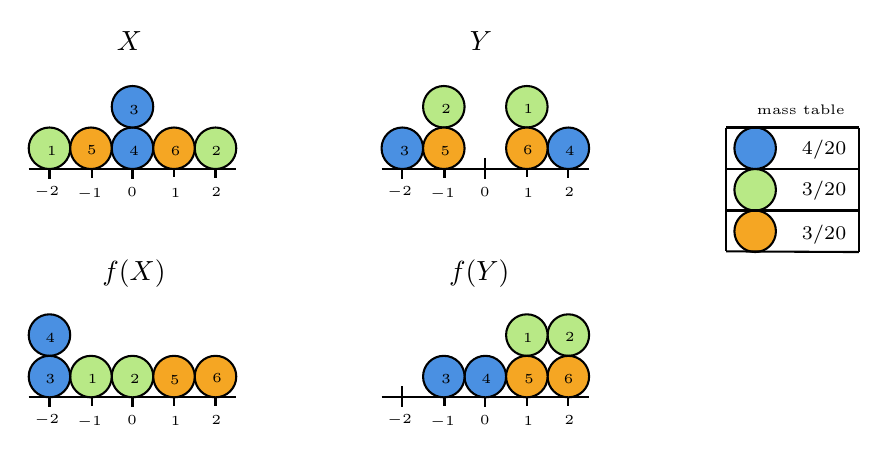
\begin{tikzpicture}[x=0.75pt,y=0.75pt,yscale=-1,xscale=1]
		%uncomment if require: \path (0,300); %set diagram left start at 0, and has height of 300
		
		%Straight Lines [id:da35193445462267636] 
		\draw    (80,130) -- (180,130) ;
		%Straight Lines [id:da9807637694958036] 
		\draw    (130,124.67) -- (130,134.67) ;
		%Straight Lines [id:da46079474054289493] 
		\draw    (110.33,124.33) -- (110.33,134.33) ;
		%Straight Lines [id:da9266328965717958] 
		\draw    (90,124.67) -- (90,134.67) ;
		%Straight Lines [id:da26812861847968716] 
		\draw    (150,124) -- (150,134) ;
		%Straight Lines [id:da21560973066226619] 
		\draw    (170,124.33) -- (170,134.33) ;
		%Shape: Circle [id:dp6385632921074851] 
		\draw  [fill={rgb, 255:red, 184; green, 233; blue, 134 }  ,fill opacity=1 ] (80,120) .. controls (80,114.48) and (84.48,110) .. (90,110) .. controls (95.52,110) and (100,114.48) .. (100,120) .. controls (100,125.52) and (95.52,130) .. (90,130) .. controls (84.48,130) and (80,125.52) .. (80,120) -- cycle ;
		%Shape: Circle [id:dp88757539189809] 
		\draw  [fill={rgb, 255:red, 184; green, 233; blue, 134 }  ,fill opacity=1 ] (160,120) .. controls (160,114.48) and (164.48,110) .. (170,110) .. controls (175.52,110) and (180,114.48) .. (180,120) .. controls (180,125.52) and (175.52,130) .. (170,130) .. controls (164.48,130) and (160,125.52) .. (160,120) -- cycle ;
		%Shape: Circle [id:dp00023416890886918118] 
		\draw  [fill={rgb, 255:red, 74; green, 144; blue, 226 }  ,fill opacity=1 ] (120,120) .. controls (120,114.48) and (124.48,110) .. (130,110) .. controls (135.52,110) and (140,114.48) .. (140,120) .. controls (140,125.52) and (135.52,130) .. (130,130) .. controls (124.48,130) and (120,125.52) .. (120,120) -- cycle ;
		%Shape: Circle [id:dp5305226281914701] 
		\draw  [fill={rgb, 255:red, 74; green, 144; blue, 226 }  ,fill opacity=1 ] (120,100) .. controls (120,94.48) and (124.48,90) .. (130,90) .. controls (135.52,90) and (140,94.48) .. (140,100) .. controls (140,105.52) and (135.52,110) .. (130,110) .. controls (124.48,110) and (120,105.52) .. (120,100) -- cycle ;
		%Shape: Circle [id:dp8678638550856308] 
		\draw  [fill={rgb, 255:red, 245; green, 166; blue, 35 }  ,fill opacity=1 ] (100,120) .. controls (100,114.48) and (104.48,110) .. (110,110) .. controls (115.52,110) and (120,114.48) .. (120,120) .. controls (120,125.52) and (115.52,130) .. (110,130) .. controls (104.48,130) and (100,125.52) .. (100,120) -- cycle ;
		%Shape: Circle [id:dp3017884596296905] 
		\draw  [fill={rgb, 255:red, 245; green, 166; blue, 35 }  ,fill opacity=1 ] (140,120) .. controls (140,114.48) and (144.48,110) .. (150,110) .. controls (155.52,110) and (160,114.48) .. (160,120) .. controls (160,125.52) and (155.52,130) .. (150,130) .. controls (144.48,130) and (140,125.52) .. (140,120) -- cycle ;
		%Straight Lines [id:da0560420025775803] 
		\draw    (250,130) -- (350,130) ;
		%Straight Lines [id:da2151747914618083] 
		\draw    (300,124.67) -- (300,134.67) ;
		%Straight Lines [id:da5495384586463741] 
		\draw    (280.33,124.33) -- (280.33,134.33) ;
		%Straight Lines [id:da7015652694438574] 
		\draw    (260,124.67) -- (260,134.67) ;
		%Straight Lines [id:da5295885469027419] 
		\draw    (320,124) -- (320,134) ;
		%Straight Lines [id:da5874340098395976] 
		\draw    (340,124.33) -- (340,134.33) ;
		%Shape: Circle [id:dp6241858667847562] 
		\draw  [fill={rgb, 255:red, 184; green, 233; blue, 134 }  ,fill opacity=1 ] (270,100) .. controls (270,94.48) and (274.48,90) .. (280,90) .. controls (285.52,90) and (290,94.48) .. (290,100) .. controls (290,105.52) and (285.52,110) .. (280,110) .. controls (274.48,110) and (270,105.52) .. (270,100) -- cycle ;
		%Shape: Circle [id:dp5883247401593619] 
		\draw  [fill={rgb, 255:red, 184; green, 233; blue, 134 }  ,fill opacity=1 ] (310,100) .. controls (310,94.48) and (314.48,90) .. (320,90) .. controls (325.52,90) and (330,94.48) .. (330,100) .. controls (330,105.52) and (325.52,110) .. (320,110) .. controls (314.48,110) and (310,105.52) .. (310,100) -- cycle ;
		%Shape: Circle [id:dp7734578621303227] 
		\draw  [fill={rgb, 255:red, 74; green, 144; blue, 226 }  ,fill opacity=1 ] (330,120) .. controls (330,114.48) and (334.48,110) .. (340,110) .. controls (345.52,110) and (350,114.48) .. (350,120) .. controls (350,125.52) and (345.52,130) .. (340,130) .. controls (334.48,130) and (330,125.52) .. (330,120) -- cycle ;
		%Shape: Circle [id:dp8014577169403472] 
		\draw  [fill={rgb, 255:red, 74; green, 144; blue, 226 }  ,fill opacity=1 ] (250,120) .. controls (250,114.48) and (254.48,110) .. (260,110) .. controls (265.52,110) and (270,114.48) .. (270,120) .. controls (270,125.52) and (265.52,130) .. (260,130) .. controls (254.48,130) and (250,125.52) .. (250,120) -- cycle ;
		%Shape: Circle [id:dp7009708547845324] 
		\draw  [fill={rgb, 255:red, 245; green, 166; blue, 35 }  ,fill opacity=1 ] (270,120) .. controls (270,114.48) and (274.48,110) .. (280,110) .. controls (285.52,110) and (290,114.48) .. (290,120) .. controls (290,125.52) and (285.52,130) .. (280,130) .. controls (274.48,130) and (270,125.52) .. (270,120) -- cycle ;
		%Shape: Circle [id:dp17515543966196323] 
		\draw  [fill={rgb, 255:red, 245; green, 166; blue, 35 }  ,fill opacity=1 ] (310,120) .. controls (310,114.48) and (314.48,110) .. (320,110) .. controls (325.52,110) and (330,114.48) .. (330,120) .. controls (330,125.52) and (325.52,130) .. (320,130) .. controls (314.48,130) and (310,125.52) .. (310,120) -- cycle ;
		%Straight Lines [id:da047683271260472004] 
		\draw    (80,240) -- (180,240) ;
		%Straight Lines [id:da06897596646315929] 
		\draw    (130,234.67) -- (130,244.67) ;
		%Straight Lines [id:da6001225133609294] 
		\draw    (110.33,234.33) -- (110.33,244.33) ;
		%Straight Lines [id:da7759787210653073] 
		\draw    (90,234.67) -- (90,244.67) ;
		%Straight Lines [id:da4808256794065102] 
		\draw    (150,234) -- (150,244) ;
		%Straight Lines [id:da15879435329235903] 
		\draw    (170,234.33) -- (170,244.33) ;
		%Shape: Circle [id:dp28723372250138723] 
		\draw  [fill={rgb, 255:red, 184; green, 233; blue, 134 }  ,fill opacity=1 ] (120,230) .. controls (120,224.48) and (124.48,220) .. (130,220) .. controls (135.52,220) and (140,224.48) .. (140,230) .. controls (140,235.52) and (135.52,240) .. (130,240) .. controls (124.48,240) and (120,235.52) .. (120,230) -- cycle ;
		%Shape: Circle [id:dp48538304745438854] 
		\draw  [fill={rgb, 255:red, 184; green, 233; blue, 134 }  ,fill opacity=1 ] (100,230) .. controls (100,224.48) and (104.48,220) .. (110,220) .. controls (115.52,220) and (120,224.48) .. (120,230) .. controls (120,235.52) and (115.52,240) .. (110,240) .. controls (104.48,240) and (100,235.52) .. (100,230) -- cycle ;
		%Shape: Circle [id:dp29386895845676997] 
		\draw  [fill={rgb, 255:red, 74; green, 144; blue, 226 }  ,fill opacity=1 ] (80,210) .. controls (80,204.48) and (84.48,200) .. (90,200) .. controls (95.52,200) and (100,204.48) .. (100,210) .. controls (100,215.52) and (95.52,220) .. (90,220) .. controls (84.48,220) and (80,215.52) .. (80,210) -- cycle ;
		%Shape: Circle [id:dp5371834929031682] 
		\draw  [fill={rgb, 255:red, 74; green, 144; blue, 226 }  ,fill opacity=1 ] (80,230) .. controls (80,224.48) and (84.48,220) .. (90,220) .. controls (95.52,220) and (100,224.48) .. (100,230) .. controls (100,235.52) and (95.52,240) .. (90,240) .. controls (84.48,240) and (80,235.52) .. (80,230) -- cycle ;
		%Shape: Circle [id:dp679780772291168] 
		\draw  [fill={rgb, 255:red, 245; green, 166; blue, 35 }  ,fill opacity=1 ] (160,230) .. controls (160,224.48) and (164.48,220) .. (170,220) .. controls (175.52,220) and (180,224.48) .. (180,230) .. controls (180,235.52) and (175.52,240) .. (170,240) .. controls (164.48,240) and (160,235.52) .. (160,230) -- cycle ;
		%Shape: Circle [id:dp09916225023407454] 
		\draw  [fill={rgb, 255:red, 245; green, 166; blue, 35 }  ,fill opacity=1 ] (140,230) .. controls (140,224.48) and (144.48,220) .. (150,220) .. controls (155.52,220) and (160,224.48) .. (160,230) .. controls (160,235.52) and (155.52,240) .. (150,240) .. controls (144.48,240) and (140,235.52) .. (140,230) -- cycle ;
		%Straight Lines [id:da005830372732677835] 
		\draw    (250,240) -- (350,240) ;
		%Straight Lines [id:da8496538110163001] 
		\draw    (300,234.67) -- (300,244.67) ;
		%Straight Lines [id:da5296637264047355] 
		\draw    (280.33,234.33) -- (280.33,244.33) ;
		%Straight Lines [id:da5680895817724656] 
		\draw    (260,234.67) -- (260,244.67) ;
		%Straight Lines [id:da07030570834807603] 
		\draw    (320,234) -- (320,244) ;
		%Straight Lines [id:da9703804817895982] 
		\draw    (340,234.33) -- (340,244.33) ;
		%Shape: Circle [id:dp5027333987636868] 
		\draw  [fill={rgb, 255:red, 184; green, 233; blue, 134 }  ,fill opacity=1 ] (330,210) .. controls (330,204.48) and (334.48,200) .. (340,200) .. controls (345.52,200) and (350,204.48) .. (350,210) .. controls (350,215.52) and (345.52,220) .. (340,220) .. controls (334.48,220) and (330,215.52) .. (330,210) -- cycle ;
		%Shape: Circle [id:dp4629972047973214] 
		\draw  [fill={rgb, 255:red, 184; green, 233; blue, 134 }  ,fill opacity=1 ] (310,210) .. controls (310,204.48) and (314.48,200) .. (320,200) .. controls (325.52,200) and (330,204.48) .. (330,210) .. controls (330,215.52) and (325.52,220) .. (320,220) .. controls (314.48,220) and (310,215.52) .. (310,210) -- cycle ;
		%Shape: Circle [id:dp7126456798766247] 
		\draw  [fill={rgb, 255:red, 74; green, 144; blue, 226 }  ,fill opacity=1 ] (290,230) .. controls (290,224.48) and (294.48,220) .. (300,220) .. controls (305.52,220) and (310,224.48) .. (310,230) .. controls (310,235.52) and (305.52,240) .. (300,240) .. controls (294.48,240) and (290,235.52) .. (290,230) -- cycle ;
		%Shape: Circle [id:dp702252322428877] 
		\draw  [fill={rgb, 255:red, 74; green, 144; blue, 226 }  ,fill opacity=1 ] (270,230) .. controls (270,224.48) and (274.48,220) .. (280,220) .. controls (285.52,220) and (290,224.48) .. (290,230) .. controls (290,235.52) and (285.52,240) .. (280,240) .. controls (274.48,240) and (270,235.52) .. (270,230) -- cycle ;
		%Shape: Circle [id:dp7540659628053352] 
		\draw  [fill={rgb, 255:red, 245; green, 166; blue, 35 }  ,fill opacity=1 ] (330,230) .. controls (330,224.48) and (334.48,220) .. (340,220) .. controls (345.52,220) and (350,224.48) .. (350,230) .. controls (350,235.52) and (345.52,240) .. (340,240) .. controls (334.48,240) and (330,235.52) .. (330,230) -- cycle ;
		%Shape: Circle [id:dp6870485382076588] 
		\draw  [fill={rgb, 255:red, 245; green, 166; blue, 35 }  ,fill opacity=1 ] (310,230) .. controls (310,224.48) and (314.48,220) .. (320,220) .. controls (325.52,220) and (330,224.48) .. (330,230) .. controls (330,235.52) and (325.52,240) .. (320,240) .. controls (314.48,240) and (310,235.52) .. (310,230) -- cycle ;
		%Shape: Circle [id:dp5522689388859041] 
		\draw  [fill={rgb, 255:red, 74; green, 144; blue, 226 }  ,fill opacity=1 ] (420,120) .. controls (420,114.48) and (424.48,110) .. (430,110) .. controls (435.52,110) and (440,114.48) .. (440,120) .. controls (440,125.52) and (435.52,130) .. (430,130) .. controls (424.48,130) and (420,125.52) .. (420,120) -- cycle ;
		%Shape: Circle [id:dp6539414929940437] 
		\draw  [fill={rgb, 255:red, 184; green, 233; blue, 134 }  ,fill opacity=1 ] (420,140) .. controls (420,134.48) and (424.48,130) .. (430,130) .. controls (435.52,130) and (440,134.48) .. (440,140) .. controls (440,145.52) and (435.52,150) .. (430,150) .. controls (424.48,150) and (420,145.52) .. (420,140) -- cycle ;
		%Shape: Circle [id:dp010055052010330856] 
		\draw  [fill={rgb, 255:red, 245; green, 166; blue, 35 }  ,fill opacity=1 ] (420,160) .. controls (420,154.48) and (424.48,150) .. (430,150) .. controls (435.52,150) and (440,154.48) .. (440,160) .. controls (440,165.52) and (435.52,170) .. (430,170) .. controls (424.48,170) and (420,165.52) .. (420,160) -- cycle ;
		%Straight Lines [id:da40237805847461217] 
		\draw    (416,110) -- (480,110) ;
		%Straight Lines [id:da7413023184354017] 
		\draw    (416,169.67) -- (480,170) ;
		%Straight Lines [id:da9392849789444075] 
		\draw    (416,110) -- (416,169.67) ;
		%Straight Lines [id:da8876656319892611] 
		\draw    (480,110) -- (480,170) ;
		%Straight Lines [id:da7468150014903507] 
		\draw    (416,130) -- (480,130) ;
		%Straight Lines [id:da07186517033445994] 
		\draw    (416,150) -- (480,150) ;
		
		% Text Node
		\draw (126,137.4) node [anchor=north west][inner sep=0.75pt]  [font=\tiny]  {$0$};
		% Text Node
		\draw (147,137.73) node [anchor=north west][inner sep=0.75pt]  [font=\tiny]  {$1$};
		% Text Node
		\draw (166.67,137.4) node [anchor=north west][inner sep=0.75pt]  [font=\tiny]  {$2$};
		% Text Node
		\draw (81.33,136.73) node [anchor=north west][inner sep=0.75pt]  [font=\tiny]  {$-2$};
		% Text Node
		\draw (102,137.73) node [anchor=north west][inner sep=0.75pt]  [font=\tiny]  {$-1$};
		% Text Node
		\draw (296,137.4) node [anchor=north west][inner sep=0.75pt]  [font=\tiny]  {$0$};
		% Text Node
		\draw (317,137.73) node [anchor=north west][inner sep=0.75pt]  [font=\tiny]  {$1$};
		% Text Node
		\draw (336.67,137.4) node [anchor=north west][inner sep=0.75pt]  [font=\tiny]  {$2$};
		% Text Node
		\draw (251.33,136.73) node [anchor=north west][inner sep=0.75pt]  [font=\tiny]  {$-2$};
		% Text Node
		\draw (272,137.73) node [anchor=north west][inner sep=0.75pt]  [font=\tiny]  {$-1$};
		% Text Node
		\draw (126,247.4) node [anchor=north west][inner sep=0.75pt]  [font=\tiny]  {$0$};
		% Text Node
		\draw (147,247.73) node [anchor=north west][inner sep=0.75pt]  [font=\tiny]  {$1$};
		% Text Node
		\draw (166.67,247.4) node [anchor=north west][inner sep=0.75pt]  [font=\tiny]  {$2$};
		% Text Node
		\draw (81.33,246.73) node [anchor=north west][inner sep=0.75pt]  [font=\tiny]  {$-2$};
		% Text Node
		\draw (102,247.73) node [anchor=north west][inner sep=0.75pt]  [font=\tiny]  {$-1$};
		% Text Node
		\draw (296,247.4) node [anchor=north west][inner sep=0.75pt]  [font=\tiny]  {$0$};
		% Text Node
		\draw (317,247.73) node [anchor=north west][inner sep=0.75pt]  [font=\tiny]  {$1$};
		% Text Node
		\draw (336.67,247.4) node [anchor=north west][inner sep=0.75pt]  [font=\tiny]  {$2$};
		% Text Node
		\draw (251.33,246.73) node [anchor=north west][inner sep=0.75pt]  [font=\tiny]  {$-2$};
		% Text Node
		\draw (272,247.73) node [anchor=north west][inner sep=0.75pt]  [font=\tiny]  {$-1$};
		% Text Node
		\draw (121,62.4) node [anchor=north west][inner sep=0.75pt]    {$X$};
		% Text Node
		\draw (291,62.4) node [anchor=north west][inner sep=0.75pt]    {$Y$};
		% Text Node
		\draw (114,172.4) node [anchor=north west][inner sep=0.75pt]    {$f( X)$};
		% Text Node
		\draw (281,172.4) node [anchor=north west][inner sep=0.75pt]    {$f( Y)$};
		% Text Node
		\draw (451,134.4) node [anchor=north west][inner sep=0.75pt]  [font=\scriptsize]  {$3/20$};
		% Text Node
		\draw (451,114.4) node [anchor=north west][inner sep=0.75pt]  [font=\scriptsize]  {$4/20$};
		% Text Node
		\draw (451,155.4) node [anchor=north west][inner sep=0.75pt]  [font=\scriptsize]  {$3/20$};
		% Text Node
		\draw (429.33,97.67) node [anchor=north west][inner sep=0.75pt]  [font=\tiny] [align=left] {mass table};
		% Text Node
		\draw (87.33,117.73) node [anchor=north west][inner sep=0.75pt]  [font=\tiny]  {$1$};
		% Text Node
		\draw (166.67,117.73) node [anchor=north west][inner sep=0.75pt]  [font=\tiny]  {$2$};
		% Text Node
		\draw (127,97.73) node [anchor=north west][inner sep=0.75pt]  [font=\tiny]  {$3$};
		% Text Node
		\draw (127,117.73) node [anchor=north west][inner sep=0.75pt]  [font=\tiny]  {$4$};
		% Text Node
		\draw (106.67,117.07) node [anchor=north west][inner sep=0.75pt]  [font=\tiny]  {$5$};
		% Text Node
		\draw (147,117.73) node [anchor=north west][inner sep=0.75pt]  [font=\tiny]  {$6$};
		% Text Node
		\draw (277,117.73) node [anchor=north west][inner sep=0.75pt]  [font=\tiny]  {$5$};
		% Text Node
		\draw (316.67,117.07) node [anchor=north west][inner sep=0.75pt]  [font=\tiny]  {$6$};
		% Text Node
		\draw (257.33,117.73) node [anchor=north west][inner sep=0.75pt]  [font=\tiny]  {$3$};
		% Text Node
		\draw (277.33,97.4) node [anchor=north west][inner sep=0.75pt]  [font=\tiny]  {$2$};
		% Text Node
		\draw (317,97.4) node [anchor=north west][inner sep=0.75pt]  [font=\tiny]  {$1$};
		% Text Node
		\draw (337,117.73) node [anchor=north west][inner sep=0.75pt]  [font=\tiny]  {$4$};
		% Text Node
		\draw (107,227.4) node [anchor=north west][inner sep=0.75pt]  [font=\tiny]  {$1$};
		% Text Node
		\draw (127.33,227.4) node [anchor=north west][inner sep=0.75pt]  [font=\tiny]  {$2$};
		% Text Node
		\draw (146.67,228.07) node [anchor=north west][inner sep=0.75pt]  [font=\tiny]  {$5$};
		% Text Node
		\draw (167,227.07) node [anchor=north west][inner sep=0.75pt]  [font=\tiny]  {$6$};
		% Text Node
		\draw (86.67,227.4) node [anchor=north west][inner sep=0.75pt]  [font=\tiny]  {$3$};
		% Text Node
		\draw (86.67,207.73) node [anchor=north west][inner sep=0.75pt]  [font=\tiny]  {$4$};
		% Text Node
		\draw (277.33,227.4) node [anchor=north west][inner sep=0.75pt]  [font=\tiny]  {$3$};
		% Text Node
		\draw (296.67,227.73) node [anchor=north west][inner sep=0.75pt]  [font=\tiny]  {$4$};
		% Text Node
		\draw (317.33,227.4) node [anchor=north west][inner sep=0.75pt]  [font=\tiny]  {$5$};
		% Text Node
		\draw (336.33,227.73) node [anchor=north west][inner sep=0.75pt]  [font=\tiny]  {$6$};
		% Text Node
		\draw (316.67,207.73) node [anchor=north west][inner sep=0.75pt]  [font=\tiny]  {$1$};
		% Text Node
		\draw (337,207.4) node [anchor=north west][inner sep=0.75pt]  [font=\tiny]  {$2$};
		
		
	\end{tikzpicture}
\end{figure}
	 Note that we can also find other Borel measurable function. For instance you can figure out a continuous function that behaves differently on positive numbers, vs. negative numbers.
\end{solution}

\begin{problem}
	Prove that if $ \set{Z_n} $ converges to $ X $ almost surely, then for each $ \epsilon>0 $ we have $ \prob(\abs{Z_n - Z}\geq \epsilon\ i.o.) = 0 $.
\end{problem}
\begin{solution}
	We start with
	\begin{align*}
		1 = \prob(Z_n\to Z) &= \prob(\bigcap_{q\in\Q^+}\set{\abs{Z_n-Z}<q\ a.a.}) \\
		&= 1 - \prob(\bigcup_{q\in\Q^+}\set{\abs{Z_n-Z}\geqq\ i.o.})
	\end{align*}
	Thus
	\[ \prob(\bigcup_{q\in\Q^+}\set{\abs{Z_n-Z}\geq\ i.o.}) = 0. \]
	Observe that for all $ \epsilon>0 $
	\[ \set{\abs{Z_n-Z}\geq\epsilon\ i.o.} \subseteq \bigcup_{q\in\Q}\set{\abs{Z_n-Z}\geq q\ i.o.}. \]
	Thus by monotonicity of the probability function we will have
	\[ \prob(\set{\abs{Z_n-Z}\geq\epsilon\ i.o.}) \leq \prob(\bigcup_{q\in\Q}\set{\abs{Z_n-Z}\geq q\ i.o.}) = 0. \]
	So
	\[  \prob(\set{\abs{Z_n-Z}\geq\epsilon\ i.o.}) = 0. \]
\end{solution}


\begin{problem}
	Let $ X_1,X_2,\cdots $ be a sequence of random variables that are independent. Then prove that \[ X_n \to X \ a.s. \implies \sum_n \prob(\abs{X_n-X}>\epsilon) < \infty. \]
\end{problem}
\begin{solution}
	We do by the proof by contrapositive. 
	We want to proof 
	$$ \exists \epsilon>0 \quad \sum_{n} \mathbb{P}(|X_n-X|>\epsilon) = \infty \implies P(X_n\to X) = 0 $$
	
	Since $X_n$'s are independent, then by Borel-Cantelli we have
	\[ \mathbb{P}(|X_n-X|>\epsilon\ i.o.) = 1. \tag{1}. \]
	This implies 
	\[ \mathbb{P}(\bigcup_{q\in \mathbb{Q}^+} \{|X_n-X|>q\ i.o.\}) = 1. \tag{2} \]
	(if this is not clear for you see the remark below)
	
	Thus
	$$ \mathbb{P}(\bigcap_{r\in\mathbb{Q}^+}\{|X_n-X|\leq q\ a.a.\}) = 0. $$
	
	which is equivalent to 
	$$ \mathbb{P}(X_n \to X) = 0. \qed $$
\end{solution}
\begin{remark}
	To see why (1) implies (2) see the below:
	$$\{|X_n-X|>\epsilon\ i.o.\} \subseteq \bigcup_{q\in \mathbb{Q}} \{|X_n-X|>q\ i.o.\}.$$
	By monotonicity of the probability measure
	$$ 1 = \mathbb{P}(\{|X_n-X|>\epsilon\ i.o.\}) \leq \mathbb{P}(\bigcup_{q\in \mathbb{Q}^+} \{|X_n-X|>q\ i.o.\}).$$
	Thus 
	$$ \mathbb{P}(\bigcup_{q\in \mathbb{Q}^+} \{|X_n-X|>q\ i.o.\}) = 1. $$
\end{remark}

\begin{problem}
	Let $ X_1,X_2,\cdots $ be a sequence of independent random variable with $ \prob(X_n=3^n) = \prob(X_n = 3^{-n}) = \frac{1}{2} $. Let $ S_n = X_1+\cdots+X_n $.
	\begin{enumerate}[(a)]
		\item Compute $ \E{X_n} $ for each $ n $.
		\item For $ n \in \N $, compute $ R_n $ defined as
		\[ R_n = \sup\set{r\in\R : \prob(\abs{S_n}\geq r) = 1}, \]
		i.e. the largest number such that $ \abs{S_n} $ is always at least $ R_n $.
	\end{enumerate}
\end{problem}
\begin{solution}
	\begin{enumerate}[(a)]
		\item Observe that $ X_n $ is a simple random variable, thus
		\[ \E{X_n} = \frac{1}{2}3^n - \frac{1}{2}3^{n} = 0. \]
		
		\item The value of $ R_n $ equal to the case where for $ S_n $ all the random variables $ X_1,X_2,\cdots, X_{n-1} $ assume their lowest value i.e. $ -3,-9,\cdots,-3^{n-1} $ respectively, and the random variable $ X_n $ assumes its largest value, i.e. $ 3^n $.
		So we will have
		\[ S_n = 3^n - (3+9+\cdots+3^{n-1}) = 3^n - \frac{3^n-3}{2} = \frac{3^n+3}{2}. \]
	\end{enumerate}
\end{solution}






